
\documentclass{beamer}
\usepackage{xparse}
\usepackage[latin1]{inputenc}
\usepackage{slashed}
\usepackage{amsmath}

\usepackage{amssymb}
\usepackage{amsfonts}
\usepackage{lmodern}
\mode<presentation> 
\usetheme{CambridgeUS}
\usepackage[english]{babel}
\usepackage{hyperref}
\usepackage{tabularx}
\usepackage{verbatim}
\usepackage{caption}
\captionsetup[figure]{labelformat=empty, font=tiny}% redefines the caption setup of the figures environment in the beamer class.



\begin{document}
\setbeamertemplate{bibliography item}{\insertbiblabel}
\title{Hyperspectral satellite imaging }
\subtitle{Digital imaging systems - 1MD130}
\author{Linus Falk}

\maketitle

%-----EXAMPLE SLIDES-----%

\begin{document}
\setbeamertemplate{caption}{\raggedright\insertcaption\par}
\begin{frame}
\frametitle{Introduction}
\begin{columns}
\begin{column}{0.5\textwidth}
\begin{itemize}
  \item Spectroscopy of reflected light from earth surface
  \begin{itemize}
    \item Passive technique
    \item Acquires images in many spectral bands so for each pixel a reflectance spectrum can be derived
    \item Important absorption features occur in the 400-2500 nm band (reflected solar radiation dominates natural EMS)
  \end{itemize}
\end{itemize}
\end{column}
\begin{column}{0.5\textwidth}  %%<--- here
\begin{center}
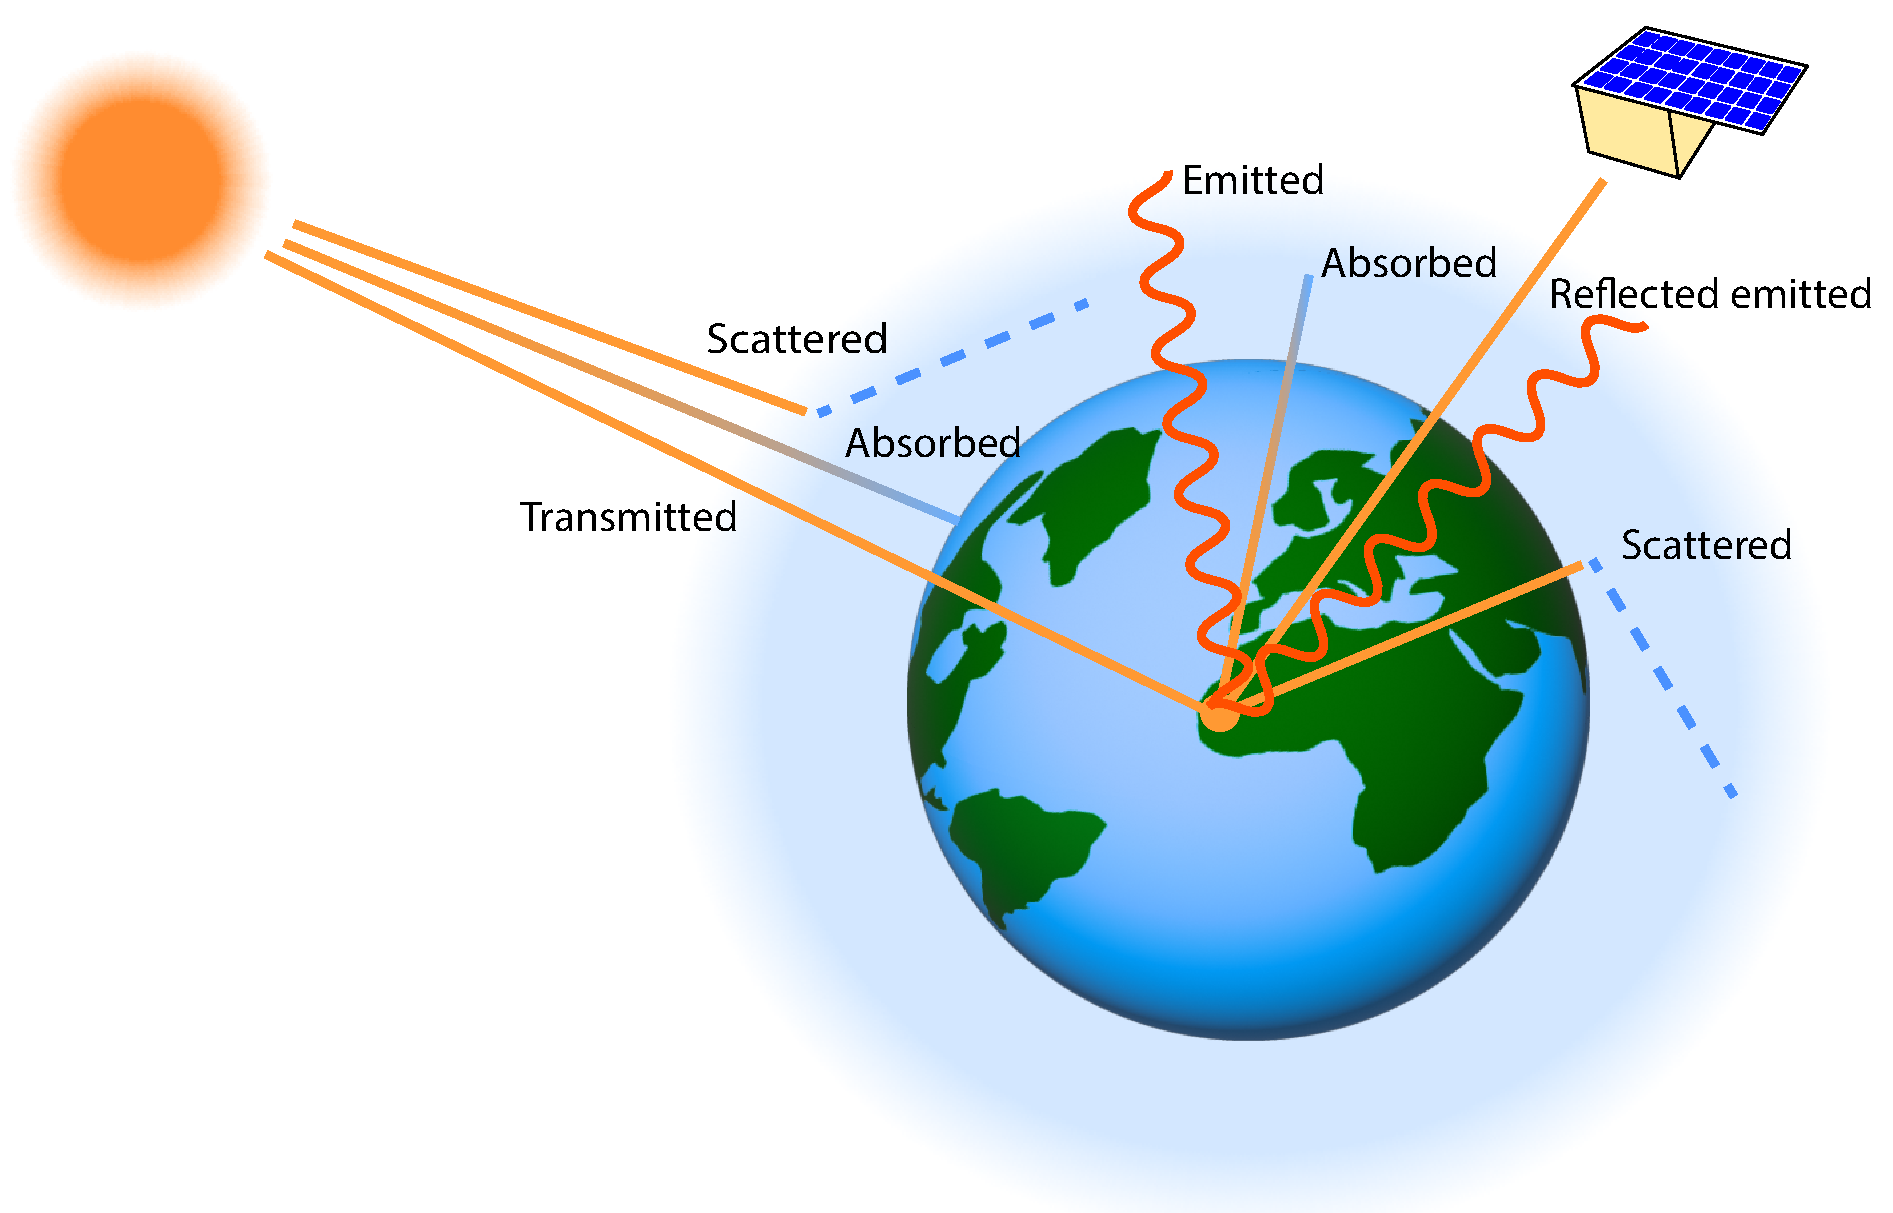
\includegraphics[width=1\textwidth]{figures/introduction_IIb.pdf}
\end{center}
\end{column}
\end{columns}
\end{frame}



% ------------------------------------------------- %

\begin{frame}
\frametitle{Introduction}
\begin{columns}
\begin{column}{0.5\textwidth}
\begin{center}
\begin{figure}
  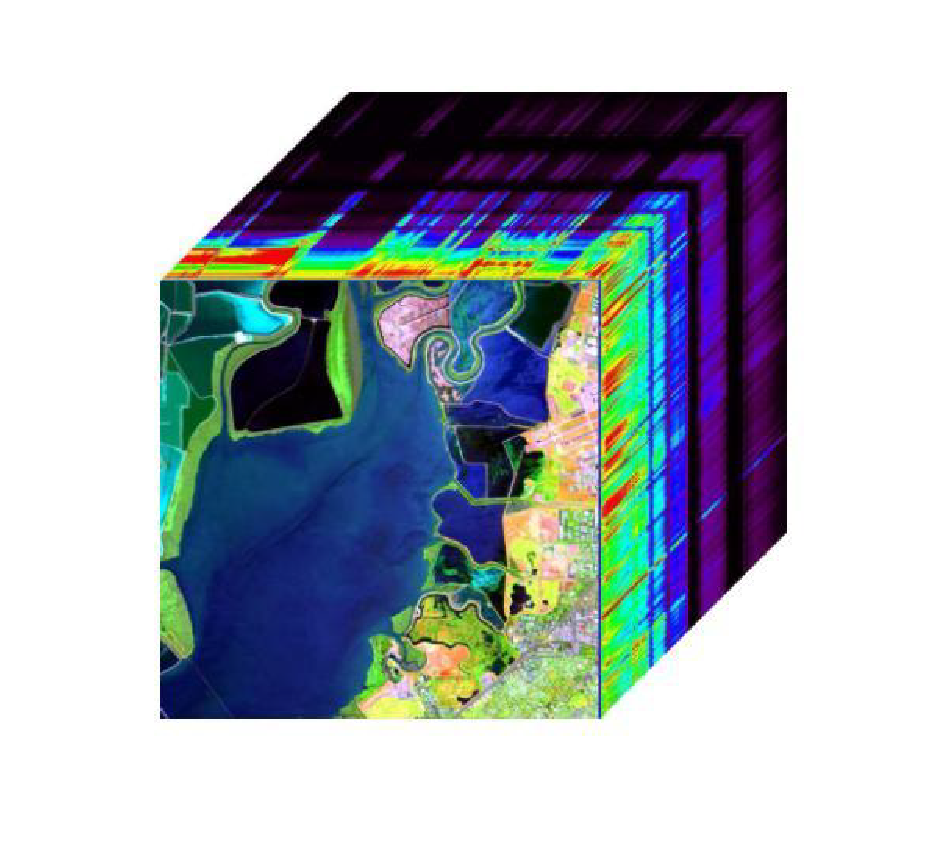
\includegraphics[width=0.8\textwidth]{figures/introduction.pdf}
  \caption{\cite{principles}}
  \end{figure}
\end{center}
        
\end{column}

        \begin{column}{0.5\textwidth}  %%<--- here
      
        \begin{center}
        \begin{figure}
        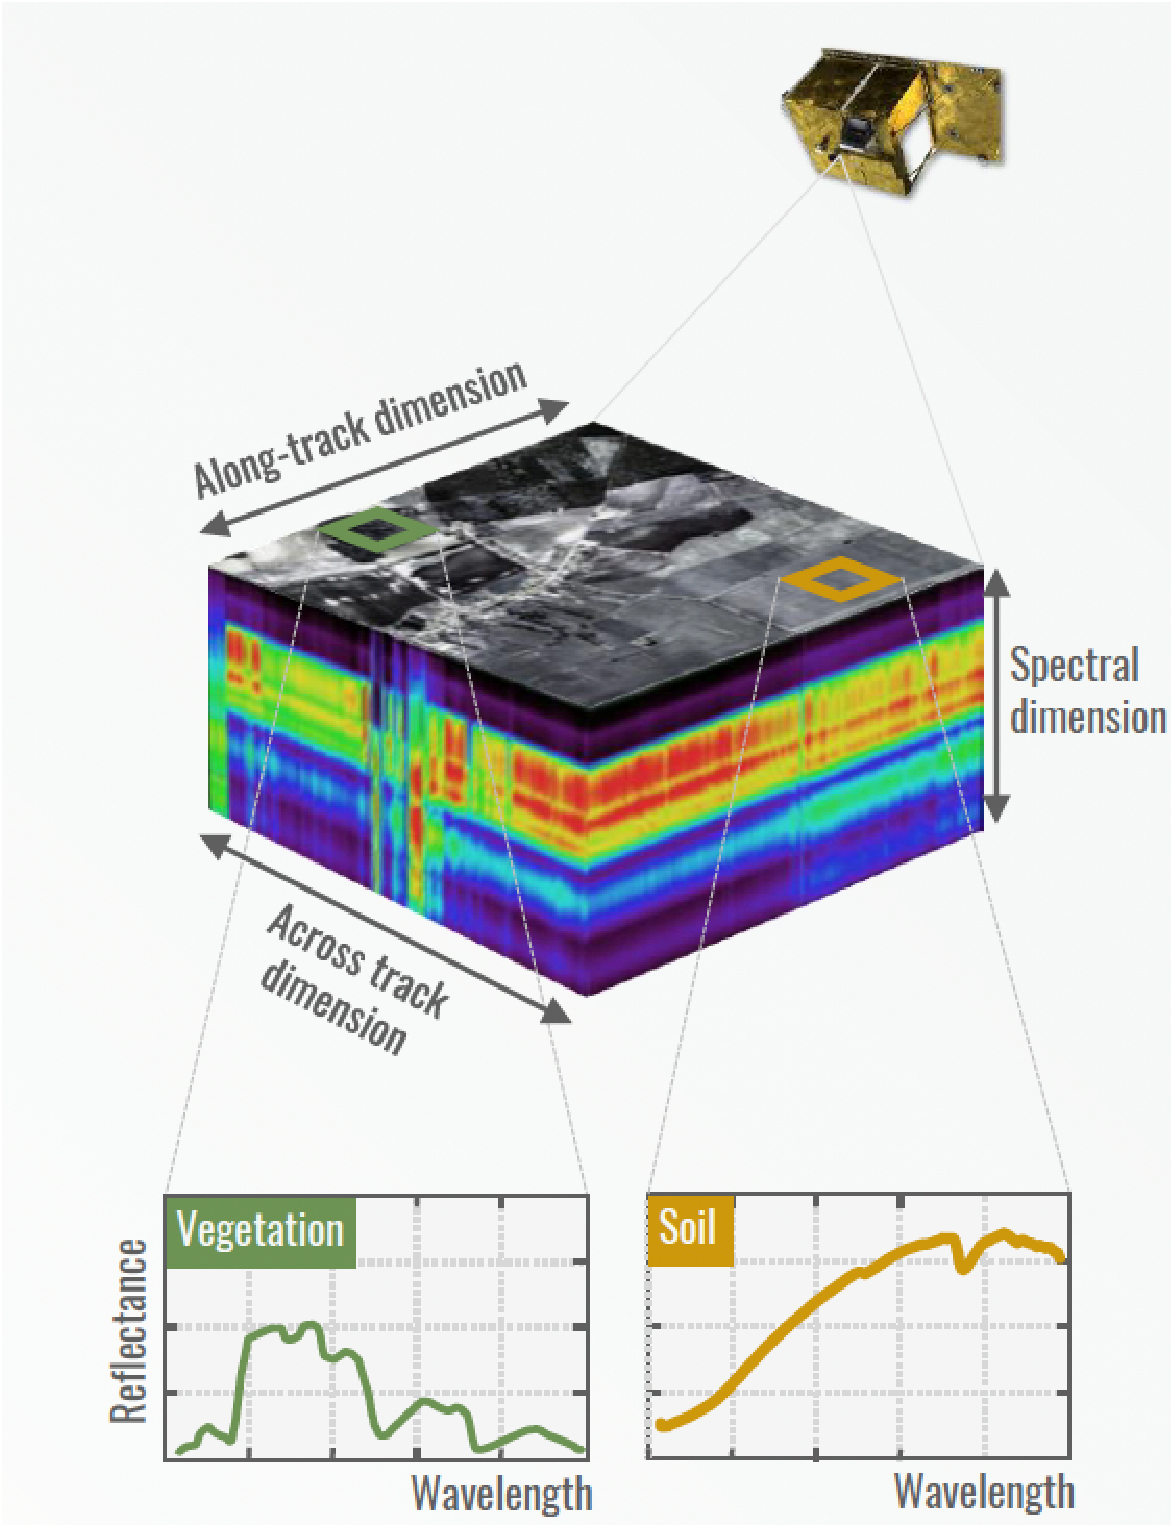
\includegraphics[width=0.8 \textwidth]{figures/eachpixel.pdf}
        \caption{\cite{sensortech}}
        \end{figure}
        \end{center}
        
        \end{column}
        \end{columns}
        \end{frame}


% ------------------------------------------------- %

\begin{frame}
\frametitle{Brief History}
\begin{columns}
\begin{column}{0.5\textwidth}
  \begin{itemize}
    \item \textbf{1660} Division of light - Sir Isaac Newton
    \item \textbf{1800-1820} Discovery of absorbtion bands - Joseph von Fraunhofer
    \item \textbf{1982} First imaging spectrometers - Jet propolsion lab (JPL)
    \item \textbf{2000} First spaceborne imaging spectrometers - NASA EO-1 
    \item \textbf{2022} Launch of EnMAP - DLR %German Aerospace Center
  \end{itemize}

  \end{column}

        \begin{column}{0.5\textwidth}  %%<--- here
        
        \begin{center}
        \begin{figure}
        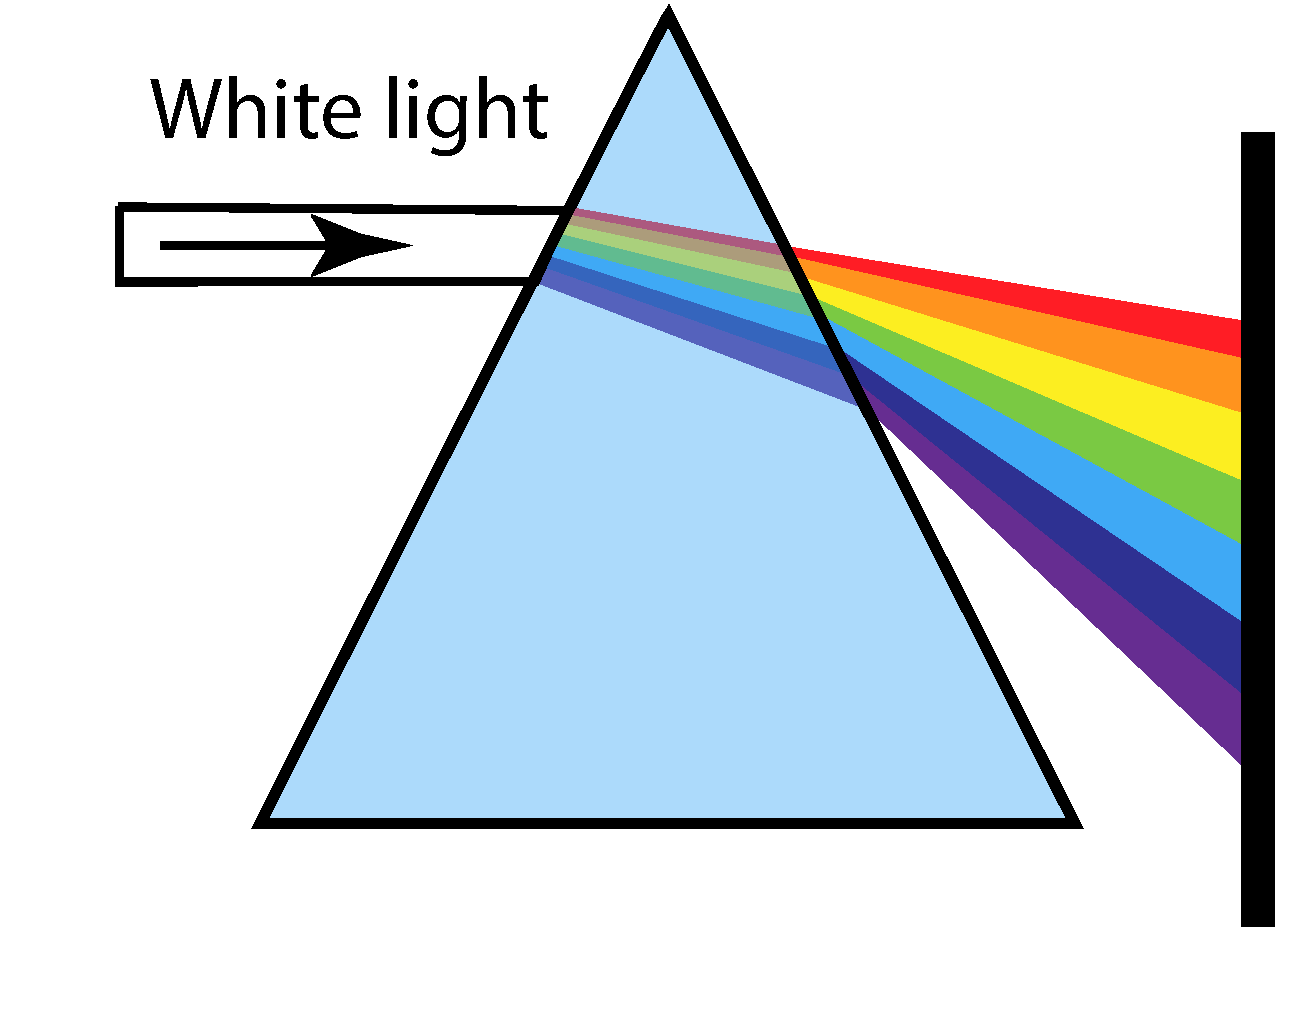
\includegraphics[width=0.6\textwidth]{figures/history2.pdf}
        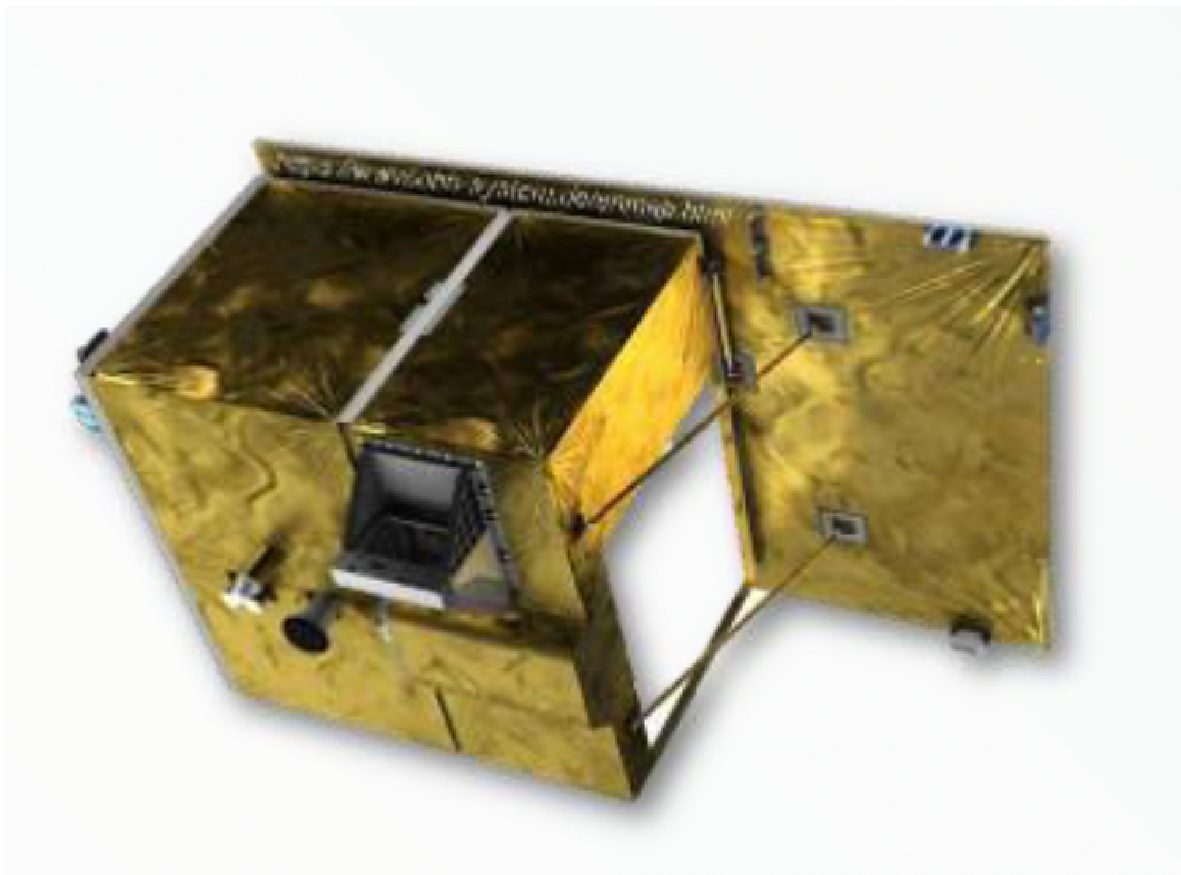
\includegraphics[width=0.6\textwidth]{figures/history3.pdf}
        \caption{\cite{sensortech}}
        \end{figure}
        \end{center}
        
        \end{column}
        \end{columns}
        \end{frame}

%https://eo-college.org/wp-content/uploads/2022/12/Basis-MOOC_offline_document_v01.pdf

\begin{comment}
\begin{itemize}
  \item +30 Years of hyperspectral satellite imaging
  \begin{itemize}
    \item Landsat-1 - \textbf{1972 NASA/JPL} (multispectral)
    \begin{itemize}
      \item Portable field reflectance spectrometers developed
    \end{itemize}
    \item For a long time was the spectral regions with atmospheric absorption seen as drawback
    \item Better algorithms and hardware made it possible to correct for this
    \item First commercial hyperspectral imaging systems for airborne use (DAIS \textbf{1989})
      \item EO1 - Hyperion sensor - \textbf{2000 NASA} %https://earthobservatory.nasa.gov/features/EO1/eo1_2.php
      \item EnMAP - \textbf{2022 DLR}
    \end{itemize}
  \end{itemize}
\end{comment}

% ------------------------------------------------- %


\begin{frame}
\frametitle{Use today \& limiting factors}
\begin{columns}
\begin{column}{0.5\textwidth}
\begin{itemize}
  \item Used in research
  \begin{itemize}
    \item Ecosystem processes
    \item Surface mineralogy
    \item Water quality
    \item Soil type and erosion, 
    \item vegetation type and more...
  \end{itemize}
  \item Global/National scale
  \begin{itemize}
    \item Limited use for private sector
  \end{itemize}
  \item Defence/military

\end{itemize}


\end{column}

        \begin{column}{0.5\textwidth}  %%<--- here
        
        \begin{center}
        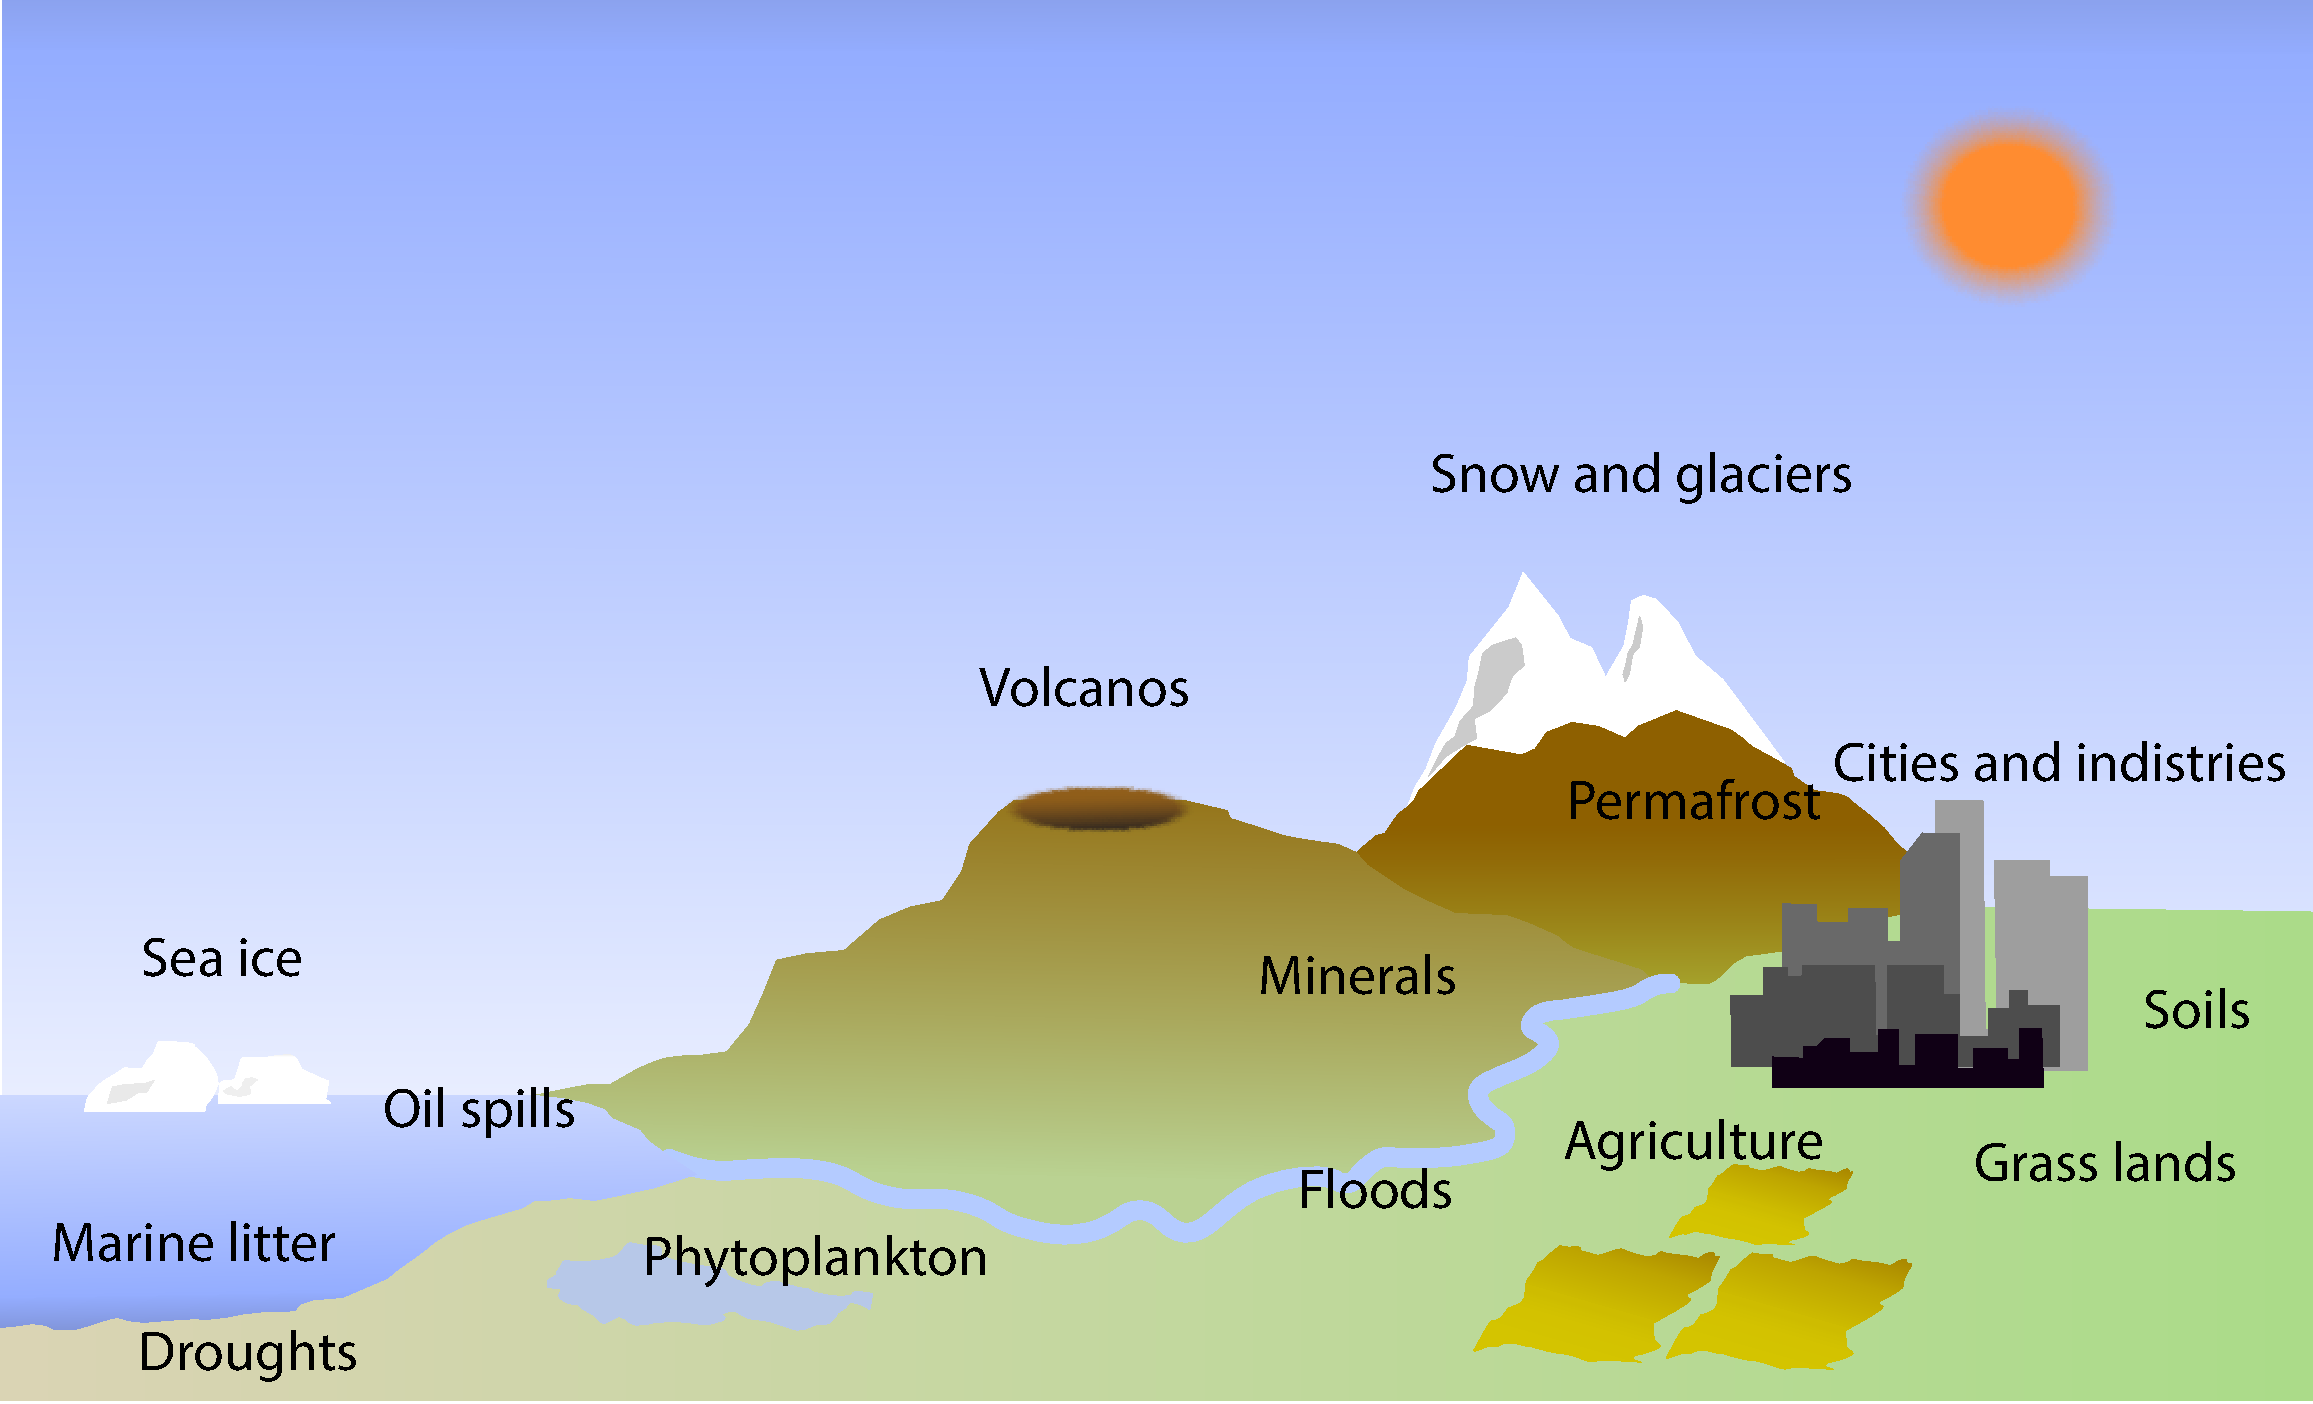
\includegraphics[width=1\textwidth]{figures/usedforb.pdf}
        \end{center}
        
        \end{column}
        \end{columns}
        \end{frame}



% ------------------------------------------------- %


\begin{frame}
\frametitle{How is the image formed}
\begin{columns}
\begin{column}{0.5\textwidth}
\begin{itemize}
  \item Scanning: 
  \begin{itemize}
    \item Push-broom
    \item Whisk-broom
  \end{itemize}
  \item Dispersive optics:
  \begin{itemize}
    \item Diffraction Grating Spectrometers
    \item Prism Spectrometers
  \end{itemize}
    \item Sensor types :  
  \begin{itemize}
    \item CMOS \& CCD - NVIR
    \item MCT (Mercury Cadmium Telluride) -SWIR (Cooled)  
  \end{itemize}

\end{itemize}


\end{column}

        \begin{column}{0.5\textwidth}  %%<--- here
        
        \begin{center}
        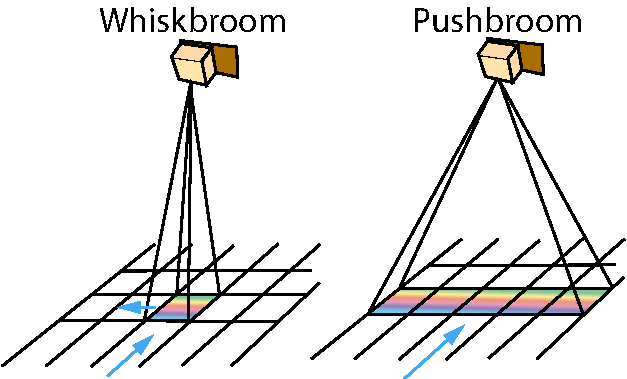
\includegraphics[width=0.8\textwidth]{figures/scan.pdf}
        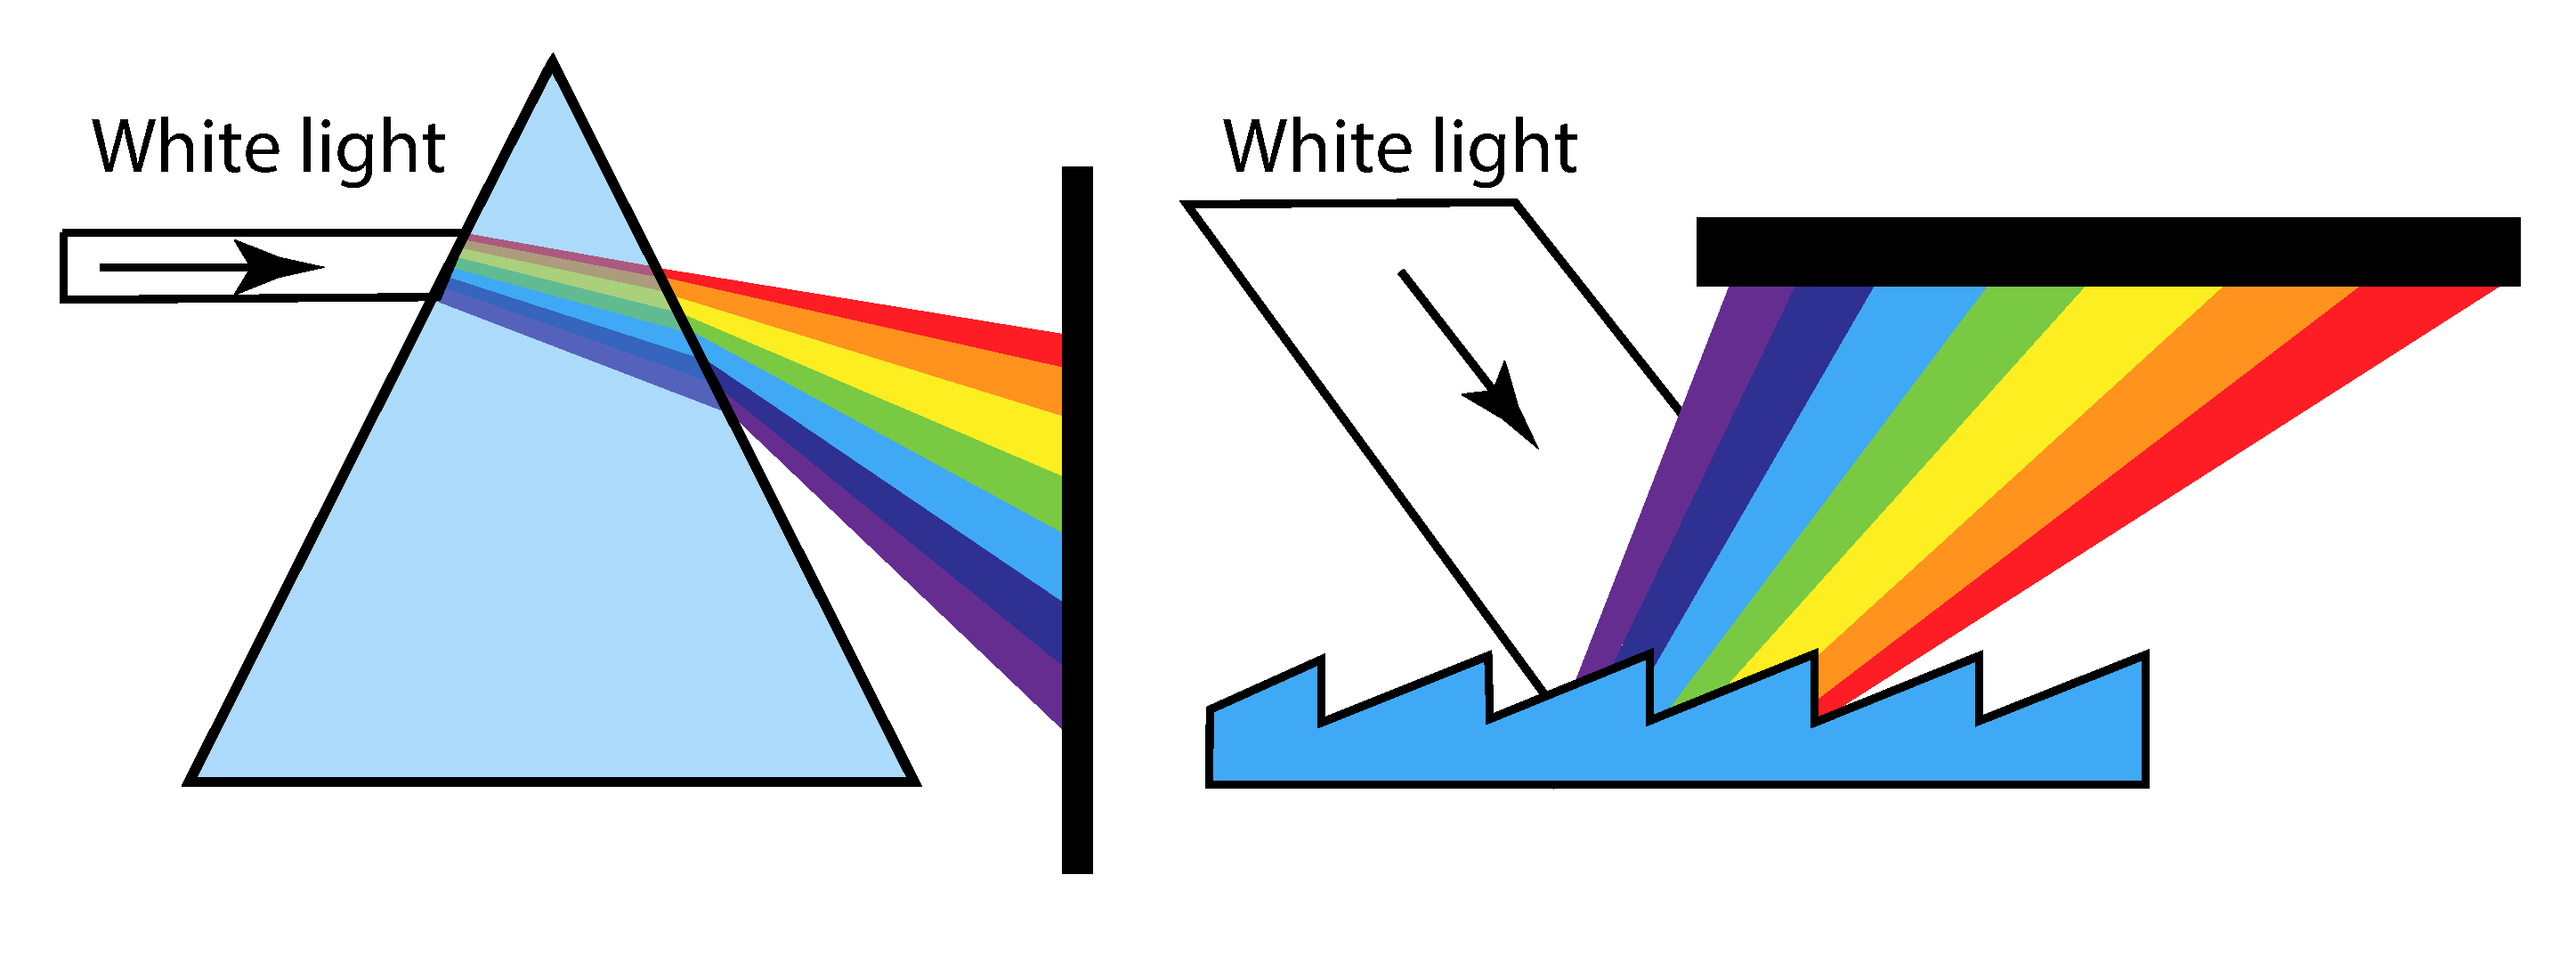
\includegraphics[width=1\textwidth]{figures/prism.pdf}
        \end{center}
        
        \end{column}
        \end{columns}
        \end{frame}


% ------------------------------------------------- %



\begin{frame}
\frametitle{How is the image formed}


    
        
        \begin{center}
        \begin{figure}
        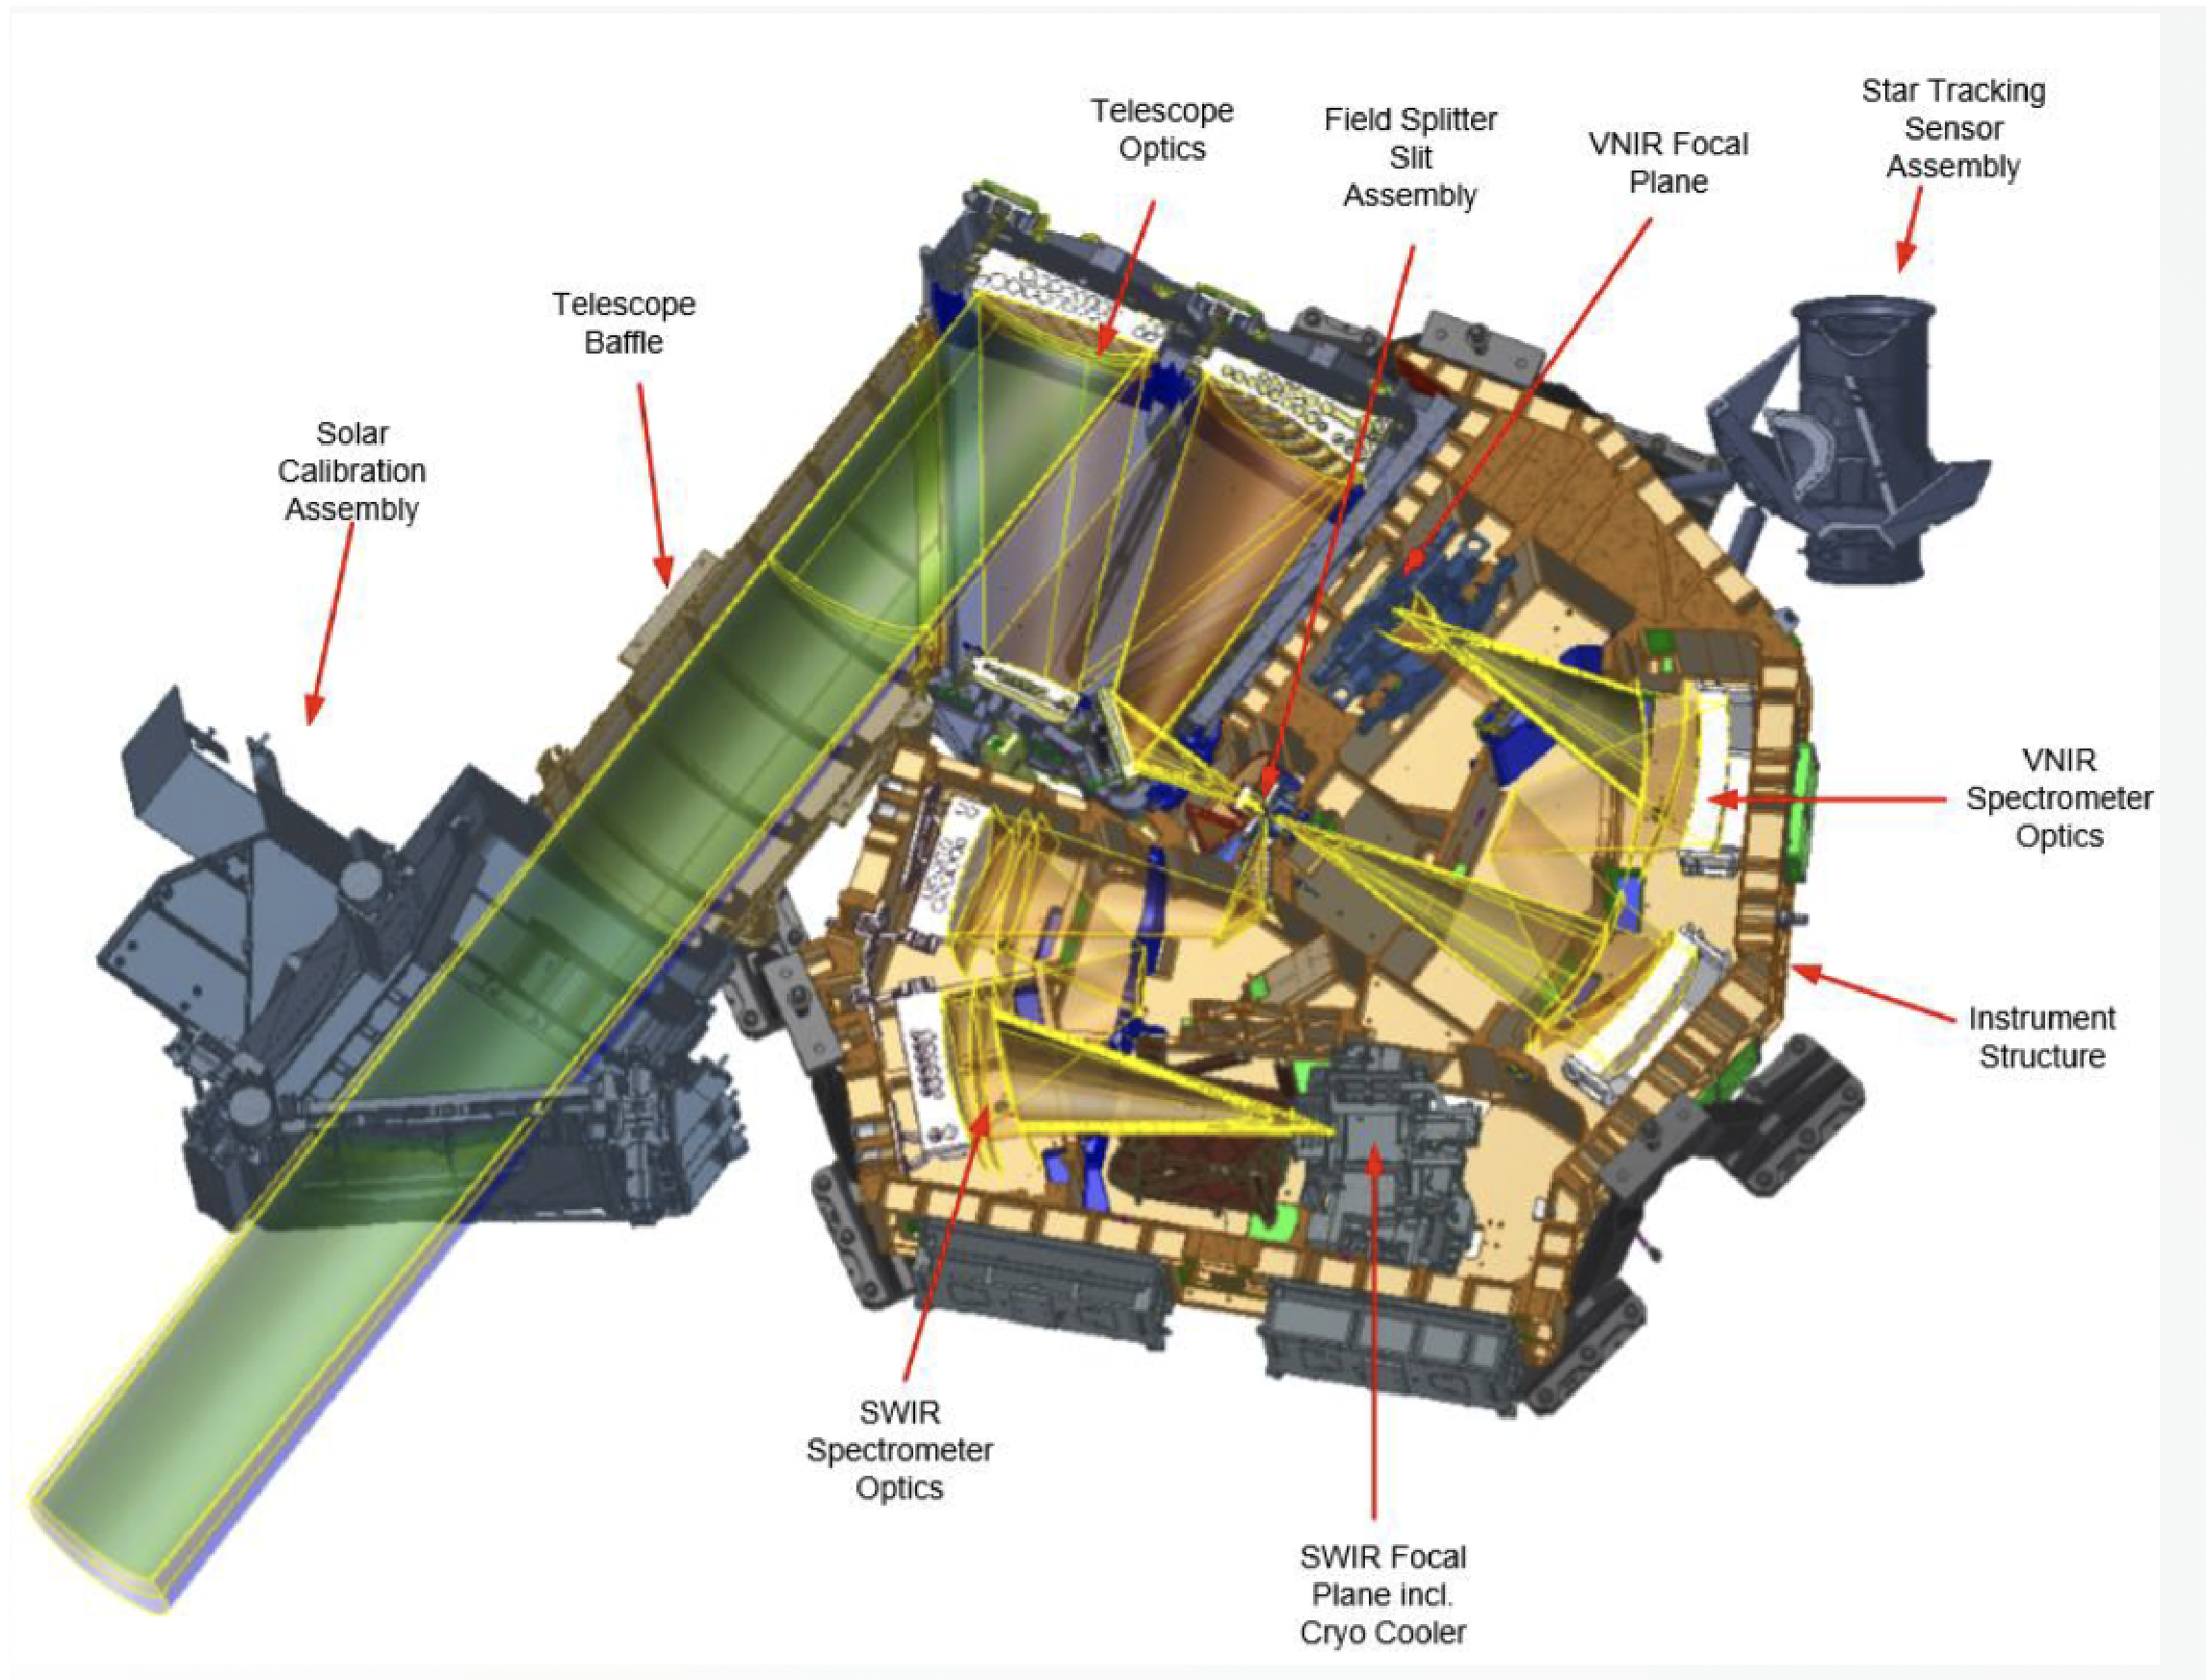
\includegraphics[width=0.7\textwidth]{figures/instrument.pdf}
        \caption{\cite{sensortech}}
        \end{figure}
        \end{center}

\end{frame}


% ------------------------------------------------- %
\begin{frame}
\frametitle{What property of the sample is imaged?}
\begin{columns}
\begin{column}{0.5\textwidth}

\begin{itemize}
  \item Interaction radiation
  \begin{itemize}
    \item Absorption 
    \item Reflection
    \item Transmission 
  \end{itemize}
    \item Absorption processes
    \begin{itemize}
      \item Electron transfer
      \item Vibrational process
    \end{itemize}
    \item Each material has a unique spectral characteristic
\end{itemize}

\end{column}

        \begin{column}{0.5\textwidth}  %%<--- here
        
        \begin{center}
        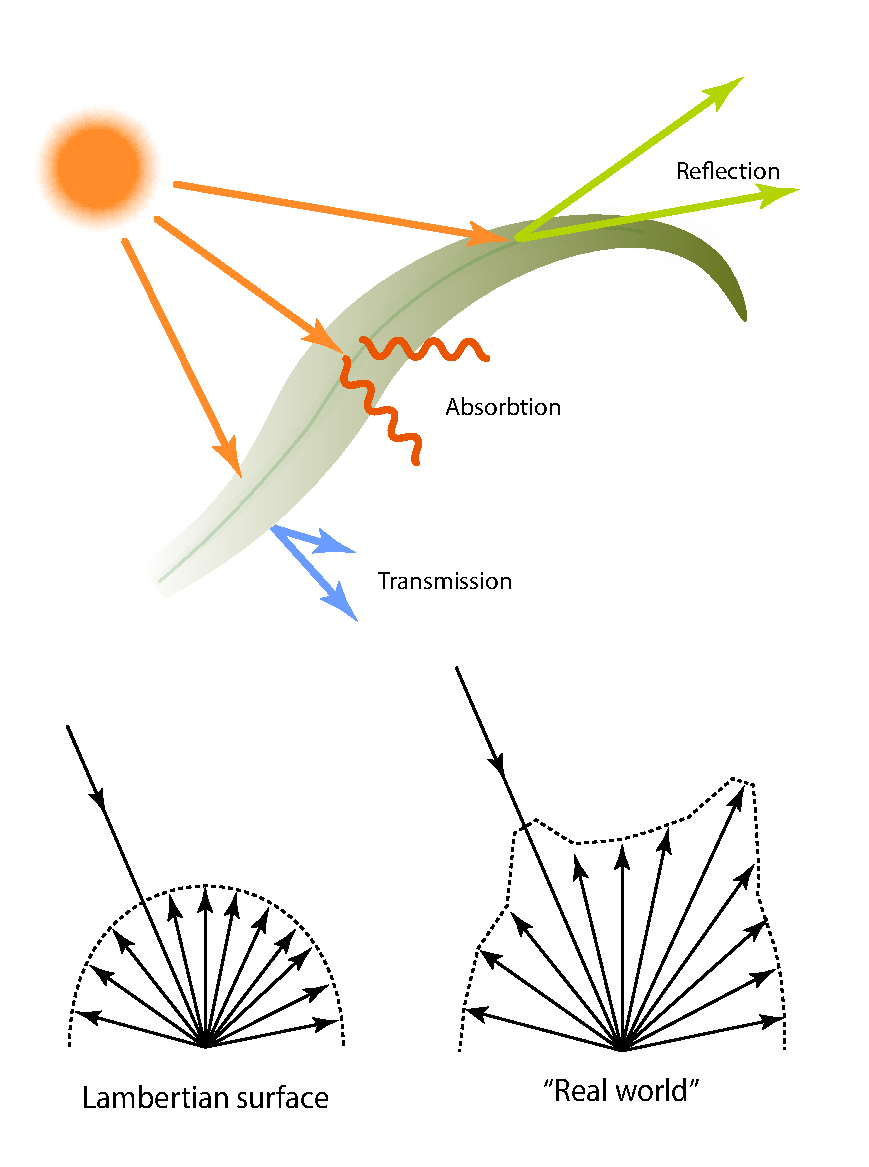
\includegraphics[width=0.7\textwidth]{figures/propertyofsampleb.pdf}
        \end{center}
        
        \end{column}
        \end{columns}
        \end{frame}


% ------------------------------------------------- %

\begin{frame}
\frametitle{What property of the sample is imaged?}
\begin{columns}
\begin{column}{0.5\textwidth}
\begin{center}
\begin{figure}
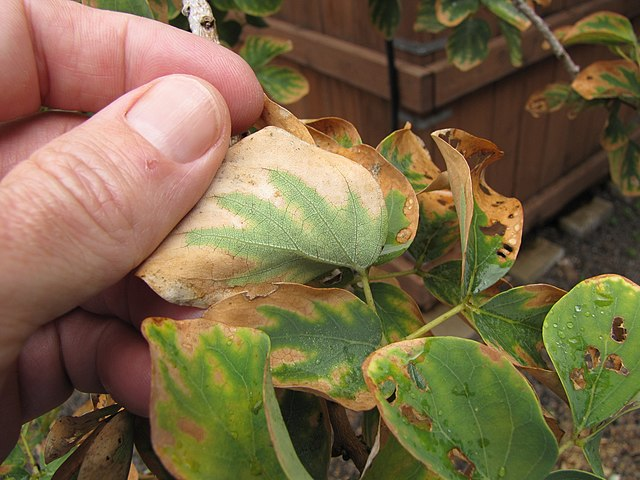
\includegraphics[width=0.8\textwidth]{figures/stressedplant.jpg}
\caption{\cite{plantstress}}
\end{figure}
\end{center}
\end{column}

        \begin{column}{0.5\textwidth}  %%<--- here
        
        \begin{center}
        \begin{figure}
        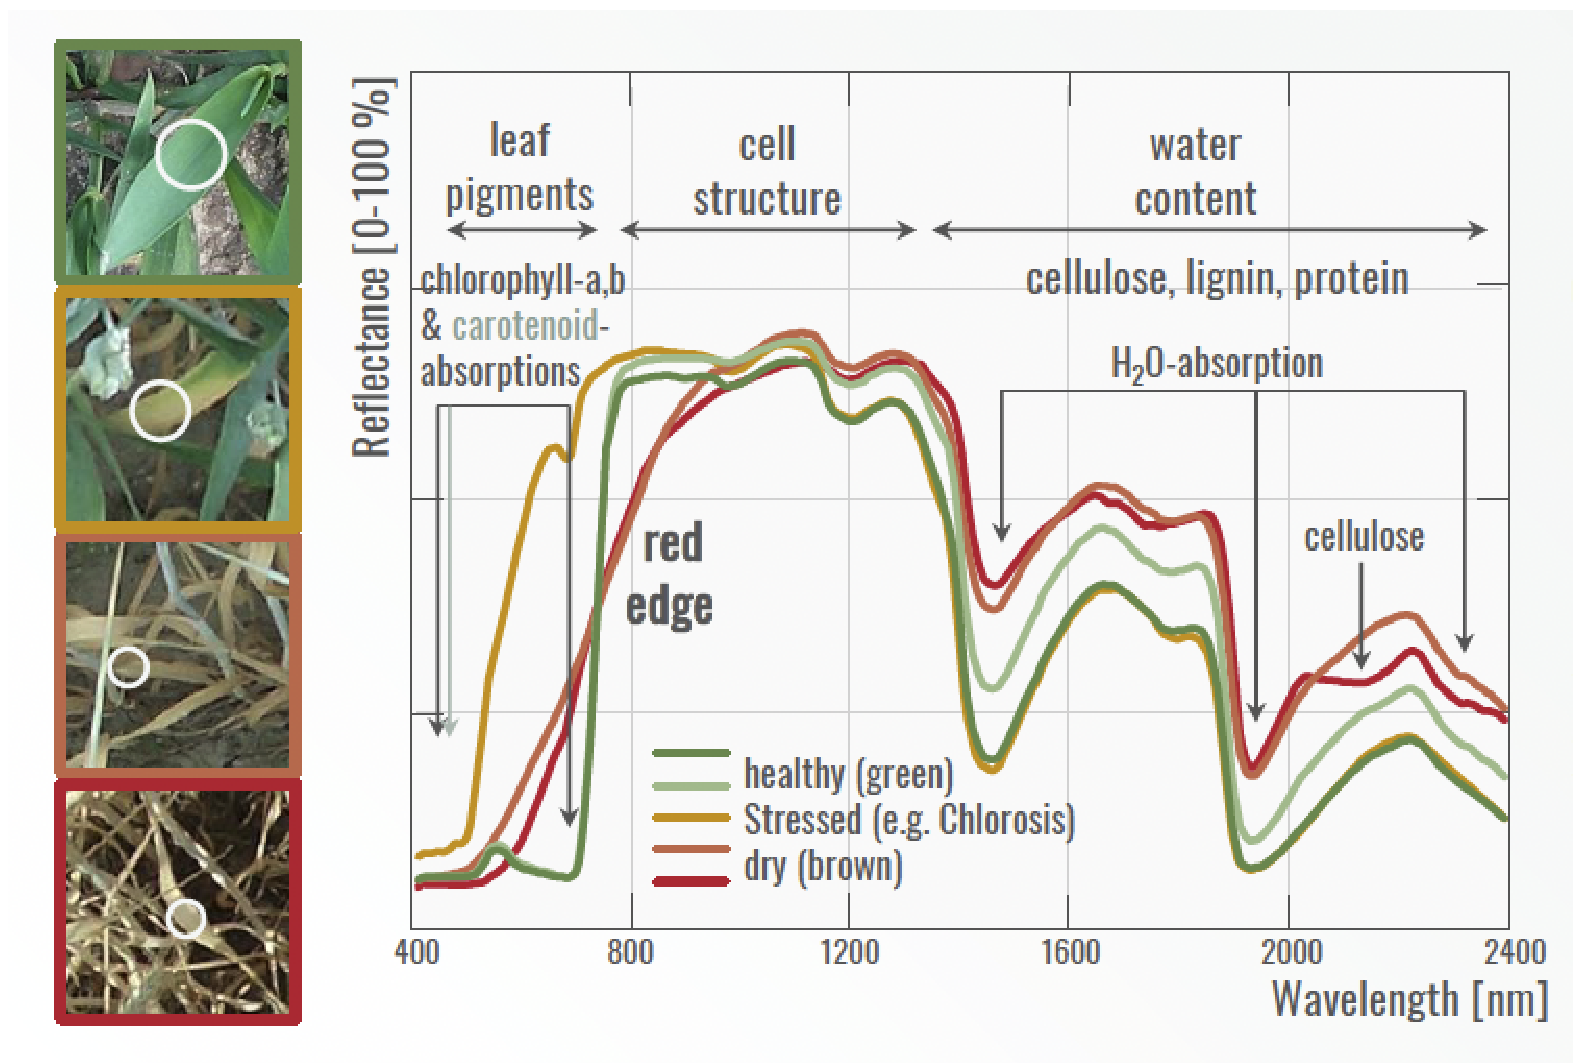
\includegraphics[width=1\textwidth]{figures/plantsignature.pdf}
        \caption{\cite{principles}}
        \end{figure}
        \end{center}
        
        \end{column}
        \end{columns}
        \end{frame}

% ------------------------------------------------- %




\begin{frame}
\frametitle{Atmospheric window}
\begin{columns}
\begin{column}{0.5\textwidth}
\begin{itemize}
  \item At surface reflectance
  \item Top-of-atmosphere radiance
  \item Atmosphere absorption
  \begin{itemize}
    \item Water vapor
    \item Carbon dioxide
    \item Ozone
  \end{itemize}
    \item Atmospheric window largely transparent 

\end{itemize}

\end{column}

        \begin{column}{0.5\textwidth}  %%<--- here
        
        \begin{center}
        \begin{figure}
        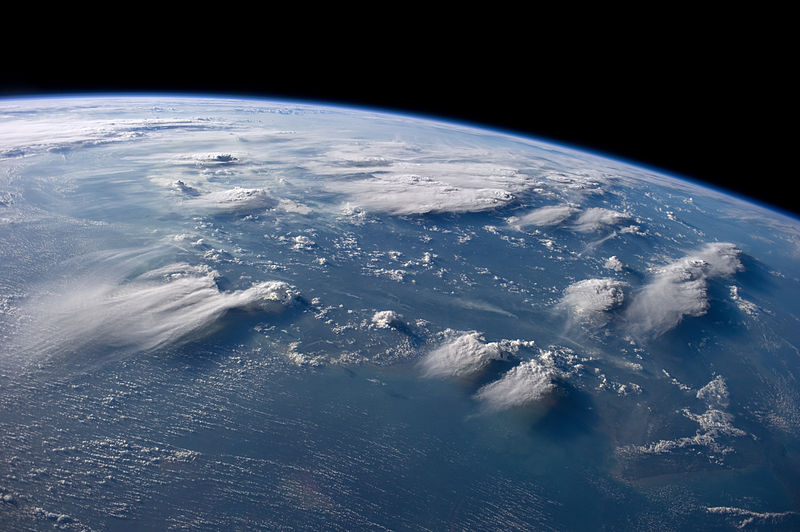
\includegraphics[width=0.7\textwidth]{figures/clouds.jpg} %https://commons.wikimedia.org/wiki/File:ISS-40_Thunderheads_near_Borneo.jpg
        \caption{\cite{clouds}}
        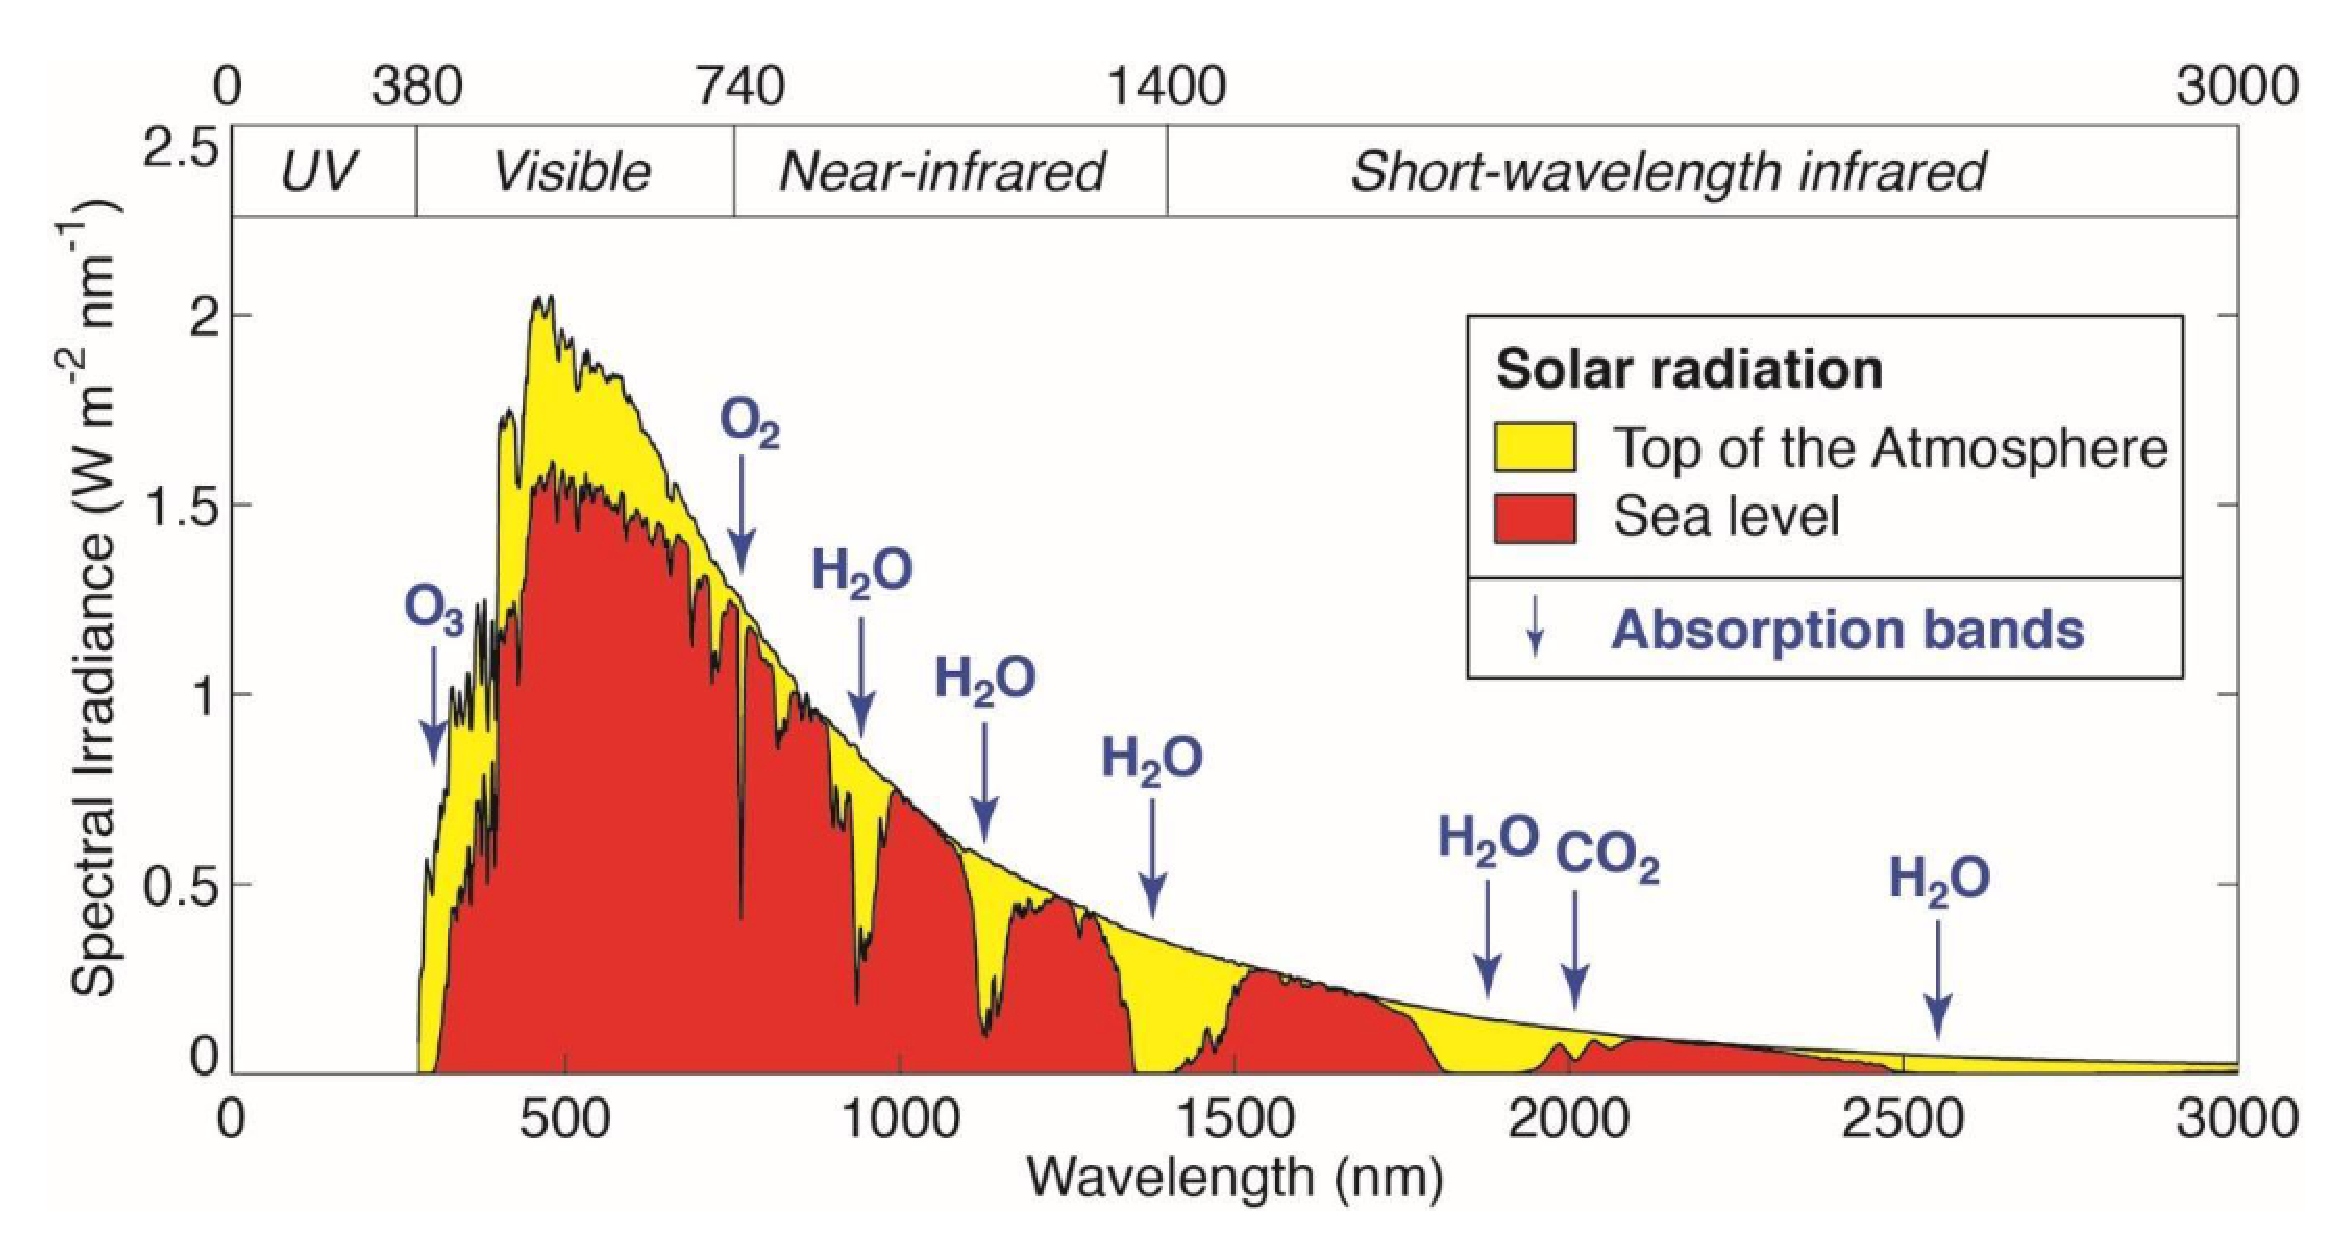
\includegraphics[width=0.8\textwidth]{figures/window.pdf} %https://www.enmap.org/data/doc/Science_Plan_EnMAP_2022_final.pdf
        \caption{\cite{enmapplan}}
        \end{figure}
        \end{center}
        
        \end{column}
        \end{columns}
        \end{frame}


% ------------------------------------------------- %



\begin{frame}
\frametitle{Resolution and sample size}
\begin{columns}
\begin{column}{0.5\textwidth}
\begin{itemize}

  \item Spatial resolution
  \begin{itemize}
    \item Field-of-view (\textbf{FOV}) and Instantaneous \textbf{FOV} (\textbf{IFOV})
    \item Ground-projected instantaneous-field-of-view (\textbf{GIFOV})
    \begin{itemize}
      \item depends on the satellite elevation and varies with the viewing angle
    \end{itemize}
    \item Across-track (ACT) and along-track (ALT) resolution
    \begin{itemize}
      \item affected by integration time and smearing effects
    \end{itemize}
  \end{itemize}
\end{itemize}

\end{column}

        \begin{column}{0.5\textwidth}  %%<--- here
        
        \begin{center}
        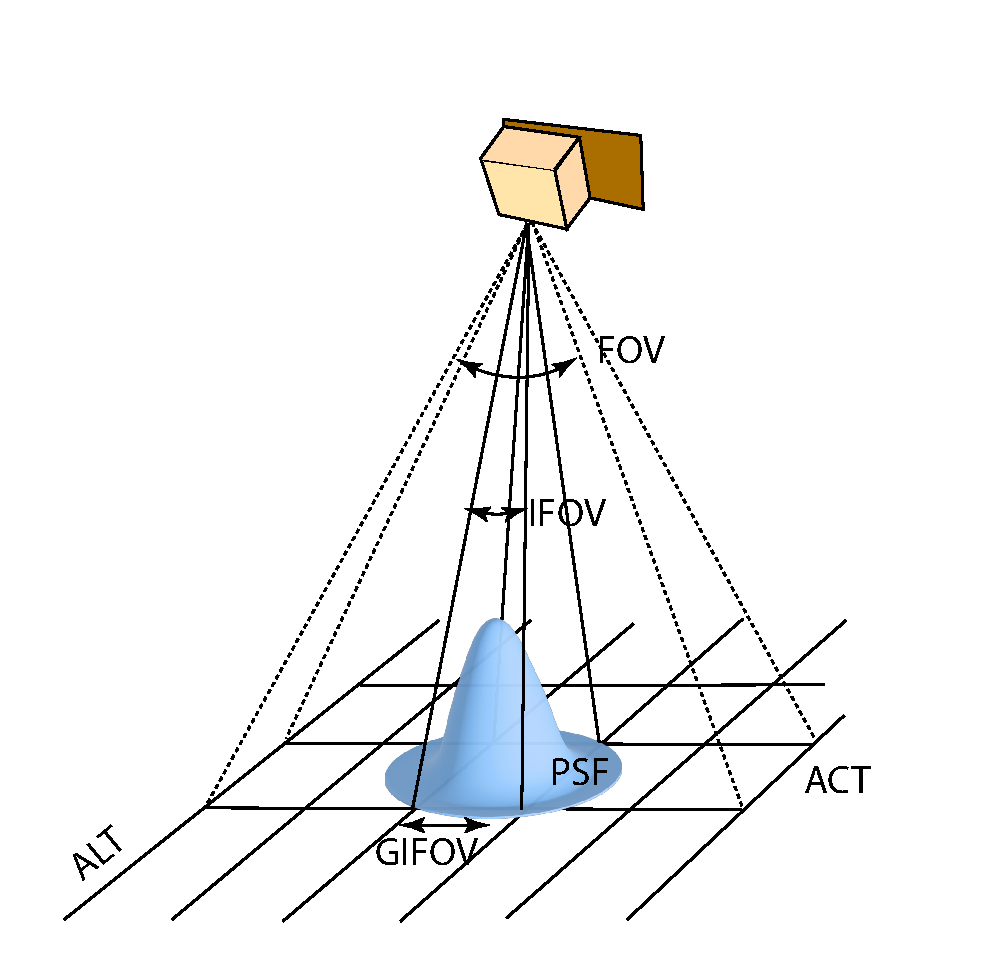
\includegraphics[width=1 \textwidth]{figures/psf.pdf}
        \end{center}
        
        \end{column}
        \end{columns}
        \end{frame}



% ------------------------------------------------- %

\begin{frame}
\frametitle{Resolution and sample size}
\begin{columns}
\begin{column}{0.5\textwidth}
\begin{itemize}
  \item Spectral resolution
  \begin{itemize}
    \item Portion of the \textbf{EMS} to which an instrument is sensitive
    \item Hyperspectral imaging - hundred of channels
  \end{itemize}
  \item Radiometric resolution
  \begin{itemize}
    \item Ability of the sensor to register differences in radiation
    \item Typically 8 and 12 bit, 
  \end{itemize}
  \item Temporal resolution
  \begin{itemize}
    \item Time between two acquisitions
    \item Depends on satellite orbit 
    \item Vary greatly depending on cloud coverage
  \end{itemize}
\end{itemize}

\end{column}

        \begin{column}{0.5\textwidth}  %%<--- here
        
        \begin{center}
        \begin{figure}
        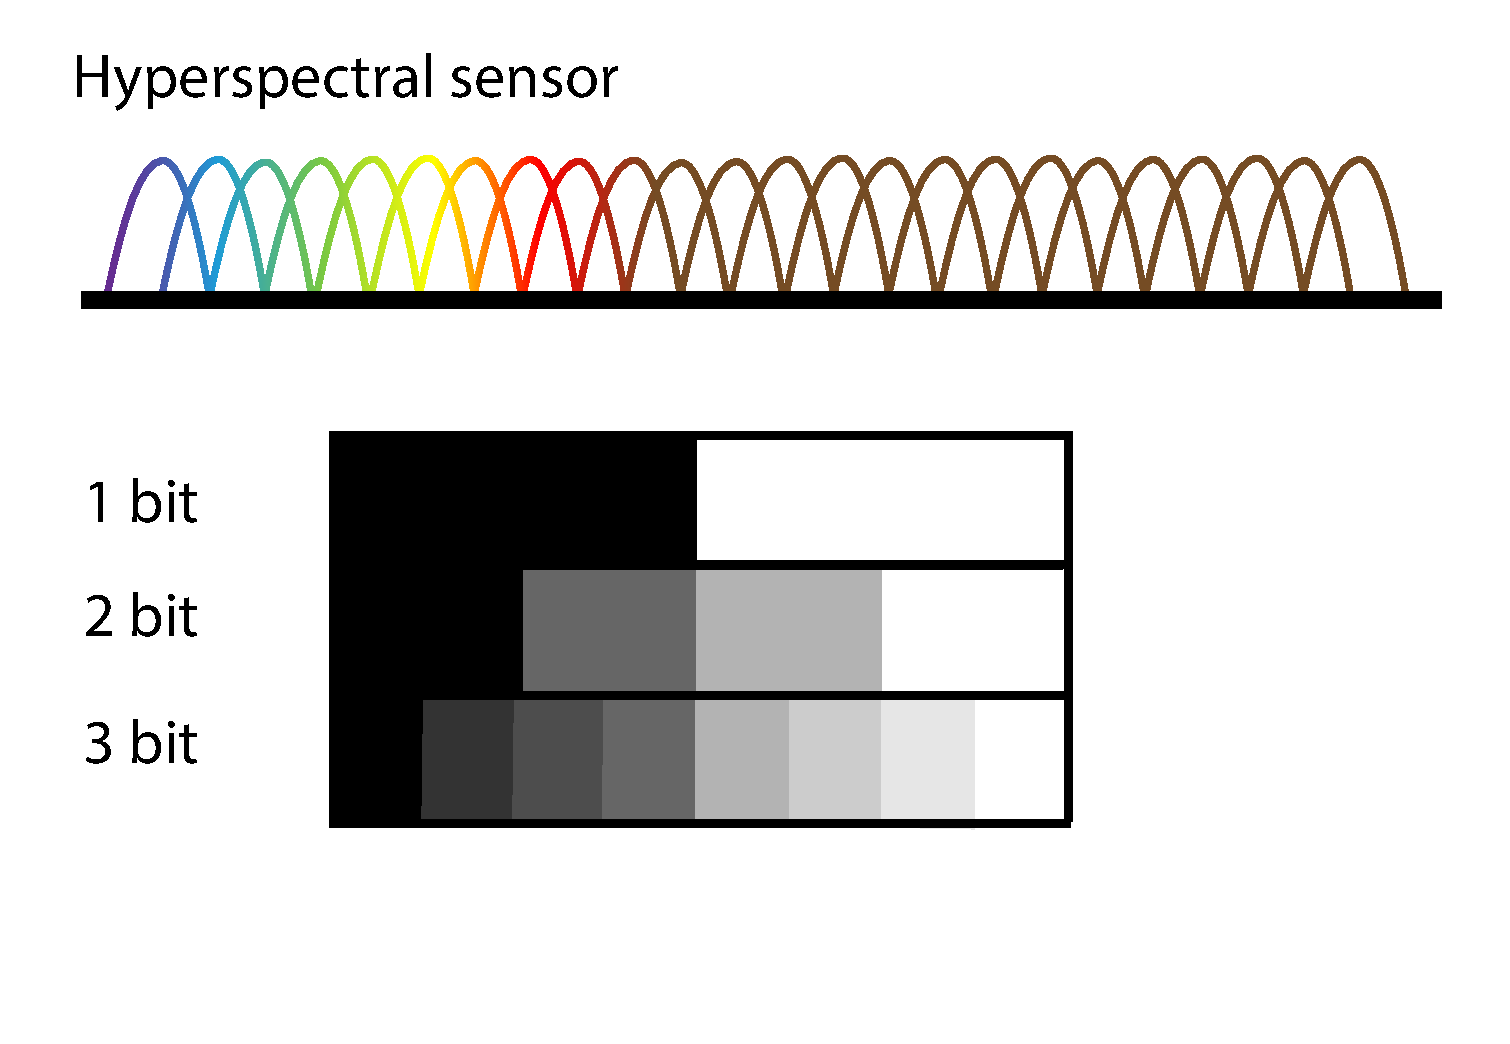
\includegraphics[width=0.7 \textwidth]{figures/bits.pdf}
        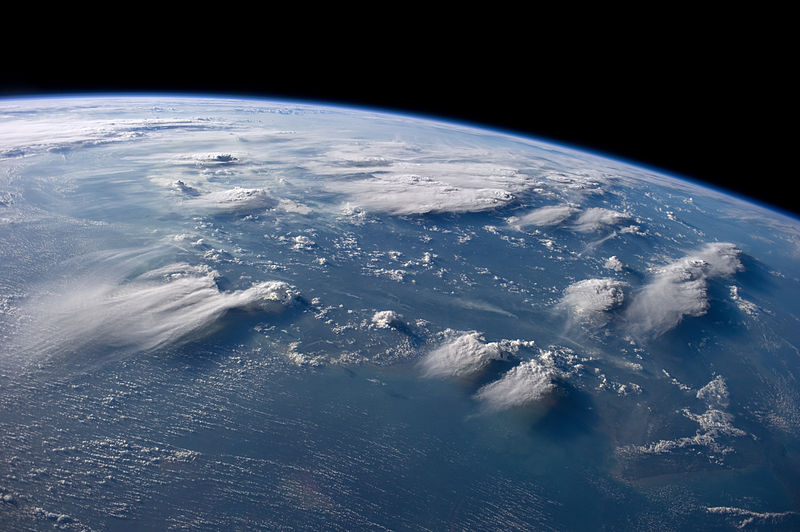
\includegraphics[width=0.8\textwidth]{figures/clouds.jpg}
        \caption{\cite{clouds}}
        \end{figure}
        \end{center}
        
        \end{column}
        \end{columns}
        \end{frame}


% ------------------------------------------------- %


\begin{frame}
\frametitle{Resolution and sample size}
\begin{center}
\begin{table}[ht!]

\begin{tabularx}{\textwidth}{XX}\hline
& \textbf{EnMAP} \\
 \textbf{Imaging principle }& Push-broom-prism\\
 \textbf{Groundsampling resolution}& 30m  \\
 \textbf{Strip lengths }& 30 - 1000km   \\
 \textbf{Spectral range}& VNIR: 420 nm - 1000 nm \newline SWIR: 900 nm - 2450 nm\\
 \raggedright
 \textbf{Mean spectral sampling distance}& VNIR: 6.5 nm \newline SWIR: 10 nm\\
 \textbf{Radiometric resolution}& 14 bit \\
 &   \\ \hline
\end{tabularx}
\caption{EnMAP in numbers}
\label{tab:tab1}
\end{table}
 \end{centering}
 \end{frame}
     



% ------------------------------------------------- %
\begin{frame}
\frametitle{Calibration & Correction}
\begin{columns}
\begin{column}{0.5\textwidth}

  \begin{itemize}
    \item Radiometric correction
    \begin{itemize}
      \item Sensor data to physical unit
      \item Use of calibration data
      \item Linear transform 
    \end{itemize}
    \item Geometric correction
    \begin{itemize}
      \item Sensor geometry to Object coordinates
    \end{itemize}
    \item Atmospheric correction 
    \begin{itemize}
      \item Atmospheric scattering
      \item Absorption effect, adjacency % https://www.researchgate.net/figure/Illustration-of-the-adjacency-effect-Most-of-the-reflectance-observed-for-the-target_fig1_260635763
      \item Illumination effect (terrain \& clouds)
    \end{itemize}
    %\item Spectral non uniformity or "Smile" correction  
    % \item Geometrically corrected (orthorectified)
  \end{itemize}

\end{column}

        \begin{column}{0.5\textwidth}  %%<--- here
        
        \begin{center}
        \begin{figure}
        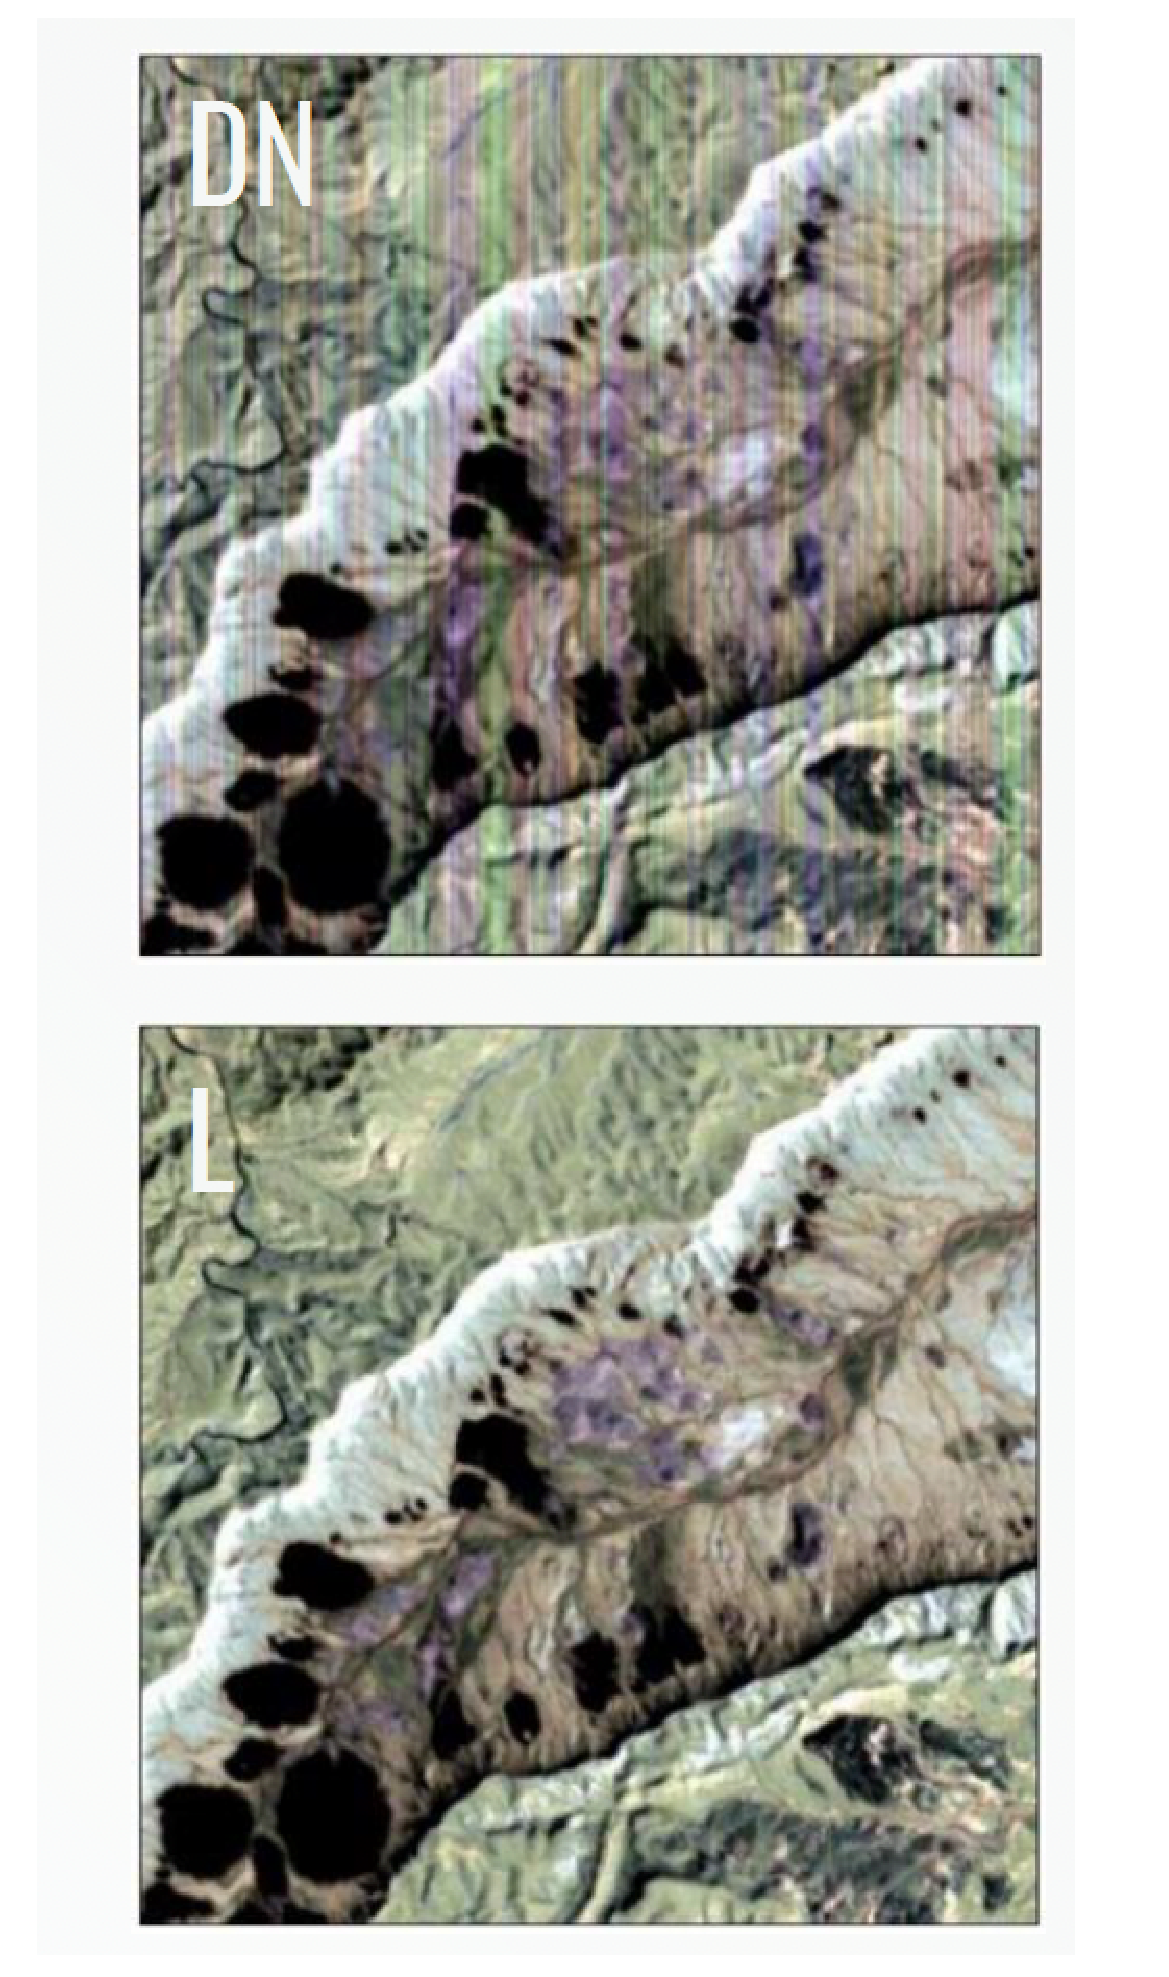
\includegraphics[width=0.6\textwidth]{figures/calcorr.pdf}
        \caption{\cite{sensortech}}
        \end{figure}
        \end{center}
        
        \end{column}
        \end{columns}
        \end{frame}


% ------------------------------------------------- %

\begin{frame}
\frametitle{Cost and limiting factors}
\begin{columns}
\begin{column}{0.5\textwidth}

\begin{itemize}
  \item Acquisition cost
  \begin{itemize}
    \item EnMAP budget:  330 million euros
    \item Five years of operations in orbit 
  \end{itemize}
  \item Data availability
  \begin{itemize}
    \item Repeat interval
    \item Historic and future data
  \end{itemize}
  \item Open source project
  \begin{itemize}
    \item EnMAPbox - QGIS
    \item Visualizing and analyzing
EnMAP data
  \end{itemize}
\end{itemize}

\end{column}

        \begin{column}{0.5\textwidth}  %%<--- here
        
        \begin{center}
        \begin{figure}
        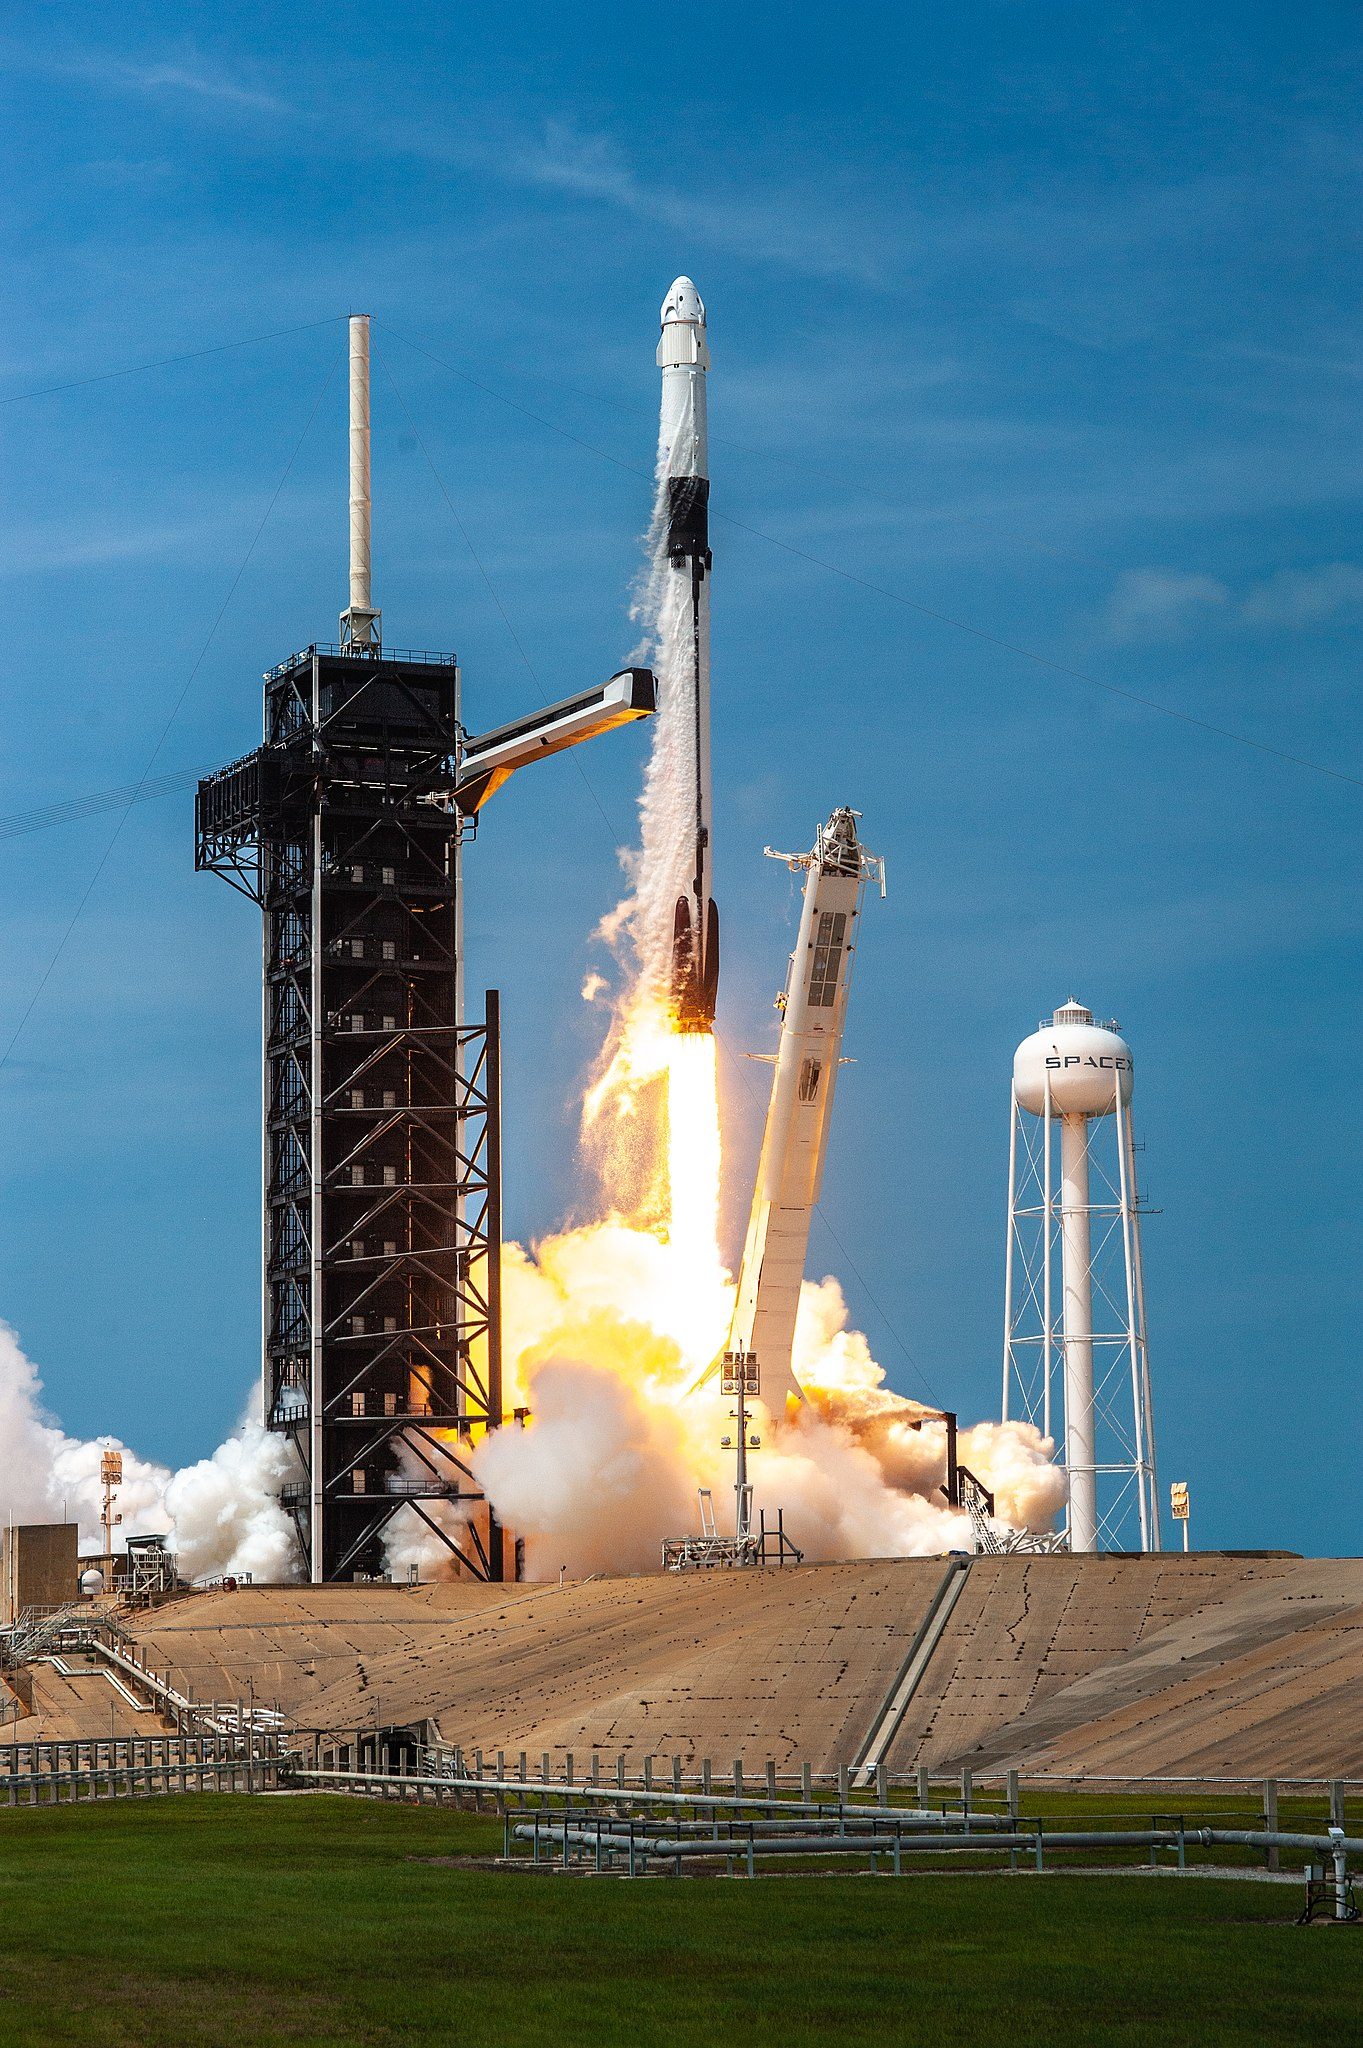
\includegraphics[width=0.7\textwidth]{figures/falcon9.jpg}
        \caption{\cite{rocket}}
        \end{figure}
        \end{center}      
        \end{column}
        \end{columns}
        \end{frame}


% ------------------------------------------------- %

\begin{frame}
\frametitle{Variants and future use}
\begin{columns}
\begin{column}{0.5\textwidth}
\begin{itemize}
  \item CubeSats - constellation of miniaturized satellites
  \begin{itemize}
    \item Better temporal resolution
  \end{itemize}
  \item Agriculture
  \item Monitor hazard and risks 
\end{itemize}

\end{column}

        \begin{column}{0.5\textwidth}  %%<--- here
        
        \begin{center}
        \begin{figure}
        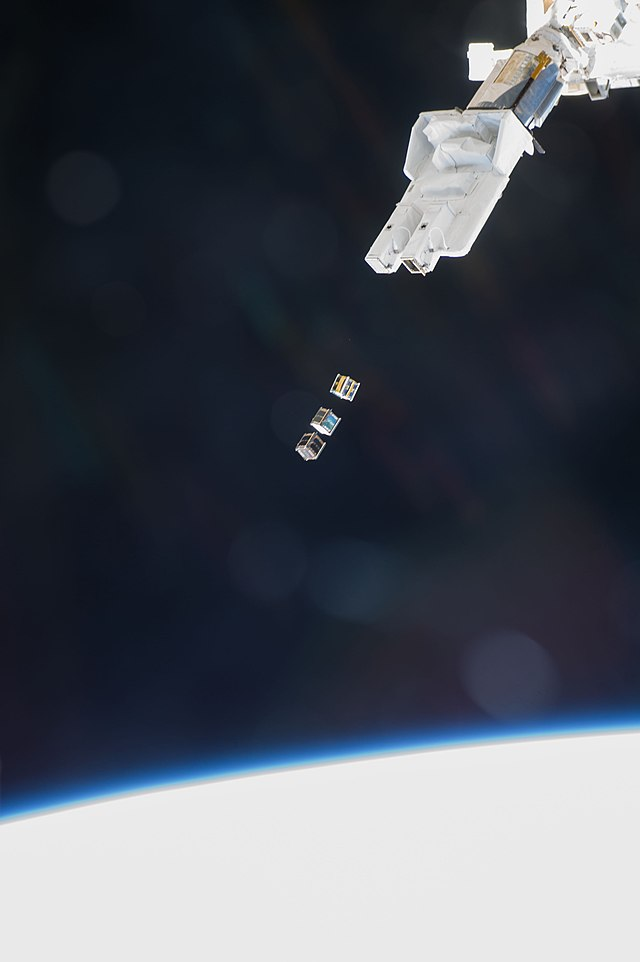
\includegraphics[width=0.7\textwidth]{figures/cubesats.jpg}
        \caption{\cite{cubes}}
        \end{figure}
        \end{center}
        
        \end{column}
        \end{columns}
        \end{frame}


% ------------------------------------------------- %



\begin{frame}
\frametitle{QGIS Demo}
\begin{columns}
\begin{column}{0.5\textwidth}


\end{column}

        \begin{column}{0.5\textwidth}  %%<--- here
        

        \end{column}
        \end{columns}
        \end{frame}


% ------------------------------------------------- %

\begin{frame}[allowframebreaks] 
\frametitle{References}
\bibliographystyle{unsrt}
\bibliography{bibliography}


\end{frame}


\end{document}


“One important artifact for some imaging spectrometers is the spectral “smile,”
also known as
spectral non uniformity or spectral aberration . It is a consequence of optical aberrations causing
the spectrometer entrance slit , representing the across track swath , to be projected as a curve
on the rectilinear detector array . This effect can be estimated in flight from atmospheric
absorption features .“ (Thompson et al.

"In the relationship of spatial and spectral
resolution, as one increases the other needs to decrease to gain the same amount
of photons on the detector. That means you either get an image with high spectral
but rather low spatial resolution (1), an image with high spatial but low spectral
resolution (2) or something in-between (both medium resolution). Sensor design tries
to avoid low SNR (3) and tries to achieve the best trade-off between spectral, spatial
resolution and high SNR for a certain application."


"Because of the strong water vapor absorption line near 22 GHz, within the microwave range, we can use microwave radiometers to measure columnar (atmospheric total) water vapor. This is a very accurate measurement due to the high signal-to-noise ratio for this measurement.  With little diurnal variation, the measurements from different satellites at the same location often agree to within a few tenths of a millimeter."

%falcon9 https://commons.wikimedia.org/wiki/File:SpaceX_Falcon_9_rocket_and_Crew_Dragon_spacecraft_lifts_off_from_Launch_Complex_39A.jpg
% cubesats https://commons.wikimedia.org/wiki/File:ISS-38_Nanosatellites_deployment_(a).jpg
% temporal https://commons.wikimedia.org/wiki/File:ISS-40_Thunderheads_near_Borneo.jpg
% stressed plant https://commons.wikimedia.org/wiki/File:Starr-120504-5544-Kanaloa_kahoolawensis-leaves_showing_stress-nursery-Maui_(24511549154).jpg#filelinks
